%% Road to VPhO 2023 Template

\documentclass[12pt]{article}
\usepackage[english]{babel}
\usepackage[T5]{fontenc}
\usepackage[top=2cm, bottom=2cm, left=2cm,right=2cm]{geometry} %%%% Margin %%%%%
\usepackage[dvipsnames]{xcolor}
\usepackage[pdftex]{graphicx}
\usepackage{wrapfig}
\usepackage{tcolorbox}
\usepackage{mathtools}
\usepackage{amsmath}
\usepackage{amssymb}
\usepackage{eqnarray}
\usepackage{siunitx}
\usepackage{array, lipsum, bibentry,fancyhdr}
\usepackage{hyperref}
\usepackage{natbib}
\setlength{\parindent}{0pt}
\usepackage{enumitem}
\usepackage[noframe]{showframe}
\usepackage{framed}
\usepackage{titling}
\usepackage{float}
\usepackage{multicol}
\usepackage{url}
\usepackage{authblk}
\usepackage{sectsty}
\usepackage{eqparbox}

%%%%%%%%%% Pictures drawing %%%%%%%%%%%%%

\usepackage{pgfplots} %%%%%% Regression %%%%
\pgfplotsset{compat = newest}
\usepackage{pgfplotstable}
\usepackage{tikz}
\usepackage{tikz-3dplot} %%%%%% Draw %%%%%%
\usepackage{tikz,tkz-euclide}
\usetikzlibrary{arrows,calc,patterns}
\usetikzlibrary{quotes,angles}
\usetikzlibrary{shapes.geometric}
\usepackage{circuitikz} %%%%% Circuit %%%%
\usetikzlibrary{decorations.pathmorphing,patterns}

\setlength{\unitlength}{1cm}

%%%%%%%%%% Ref & Hyperlink %%%%%%%%%%%%%
\usepackage{url}
\usepackage{hyperref}
\usepackage{natbib}
\hypersetup{
	colorlinks=true,
	linkcolor=blue,
	filecolor=blue,      
	urlcolor=blue,
    citecolor=blue,
	pdftitle={Overleaf Example},
	pdfpagemode=FullScreen,
}

%%%%%%%%%% Set Counter and Reference Equation %%%%%%%%%%

\usepackage{xassoccnt}
\newcounter{totalequations}
\DeclareAssociatedCounters{equation}{totalequations}
\let\theOldHequation\theHequation
\renewcommand{\theHequation}{\theOldHequation::\number\value{totalequations}}

%%%%%%%%%% Header & Footer %%%%%%%%%%%%%

\setlength{\headheight}{10mm}
\RequirePackage{fancyhdr}  % Needed to define custom headers/footers
\RequirePackage{lastpage}  % Number of pages in the document
\pagestyle{fancy}          % Enables the custom headers/footers
% Headers
\lhead{\includegraphics[width=.8in]{xPhO.png}}%
\chead{}%
\rhead{\small\sffamily\bfseries{Lời giải hướng tới VPhO 42} --- \thepage/\pageref{LastPage}}
% Footers
\lfoot{}%
\cfoot{}%
\rfoot{}%
\renewcommand{\headrulewidth}{1pt}% % header rule
\renewcommand{\footrulewidth}{1pt}% % footer rule

% \pagestyle{fancy}
% 	\fancyhead[L]{\empty}
% 	\fancyhead[R]{\empty}
% 	\fancyhead[C]{\empty}
% 	\fancyfoot[C]{\empty}
% 	\fancyfoot[L]{\empty}
% 	\renewcommand{\headrulewidth}{0pt}
% 	\fancyfoot[C]{\normalcolor{\thepage/\pageref{LastPage}}}
% 	\setcounter{page}{1}

%%%%%%%%%% Color setup %%%%%%%%%%%%%

\RequirePackage{xcolor}
\definecolor{wsdred}{HTML}{8E1728}
\definecolor{wsdgrey}{HTML}{75787B}
\renewcommand{\normalcolor}{\color{wsdred}}
\colorlet{ColorOr}{white}

\begin{document}

%% Title %%
{\fontsize{50}{24}\fontfamily{phv}\fontseries{b}
\LARGE \normalcolor{ \textbf{Lời giải hướng tới VPhO 42} } }

\textcolor{blue}{\textbf{\textit{Câu lạc bộ vật lý xPhO}}}

%%%%
\vspace{5mm}

{\normalcolor \textbf{CÂU 1. (4.0 điểm)}}\vspace{1.5mm}

\setcounter{equation}{0}
%Bổ sung lệnh vẽ lò xo
\usetikzlibrary{patterns,snakes}
\tikzstyle{spring}=[line width=0.8,blue!7!black!80,snake=coil,segment amplitude=5,segment length=5,line cap=round]

\textbf{Khối lượng âm...}

% Vào đầu thế kỷ XXI, một số nghiên cứu mới về một loại vật liệu nhân tạo được tạo bởi các cấu trúc tuần hoàn như những mạng tinh thể được gọi là \textit{metamaterial} đã mang tới một số tính chất kỳ lạ mà vật liệu tự nhiên không thể có được. Trong đó, ở lĩnh vực cơ học, loại siêu vật liệu này cho phép ta thu được "khối lượng hiệu dụng âm", "hệ số Poisson âm", "suất Young âm",... tạo ra nhiều tiềm năng ứng dụng cho các phòng cách âm hoàn hảo, siêu thấu kính,... Trong bài toán này, ta sẽ khảo sát mô hình "khối lượng trong khối lượng" (mass-in-mass model) và hiện tượng khối lượng âm của loại vật liệu này.
Ở thế giới bình thường của chúng ta, khối lượng âm là điều không tưởng. Trong một số mô hình truyền sóng cơ học, khối lượng hiệu dụng của các thành phần trong mạng tinh thể nhân tạo có thể âm và đưa đến những tính chất thú vị. Một trong những mô hình đơn giản hóa và tiêu biểu của khối lượng hiệu dụng âm là mô hình "khối lượng trong khối lượng" (mass-in-mass model).

\begin{enumerate}
\item \textbf{Mô hình mạng nguyên tử tinh thể và sóng đàn hồi.} \\
Xét một mạng tinh thể một chiều gồm các hạt khối lượng $m$ đặt cách đều nhau một khoảng $L$ như hình \ref{fig1_negative_mass}. Xem như mỗi hạt "nguyên tử" trong mạng chỉ tương tác với hai hạt liền kề nó và tương tác này tương đương với một lò xo độ cứng $k$, độ dài tự nhiên $L$. Với hạt thứ $n$ trong mạng tinh thể, vị trí cân bằng của hạt này là tại $x_n=nL$. Ta ký hiệu li độ của hạt thứ $n$ này so với vị trí cân bằng là $u_n$.

\begin{center}
\begin{tikzpicture}
    \draw[spring] (0.3,0)--++(1.4,0);
    \draw[spring] (2.3,0)--++(1.4,0);
    \draw[spring] (4.3,0)--++(1.4,0);
    \draw[spring] (6.3,0)--++(1.4,0);
    \draw[spring] (8.3,0)--++(1.4,0);
    \draw[spring] (10.3,0)--++(1.4,0);
    \draw[dashed] (-0.3,0)--(0.3,0) (11.7,0)--(12.3,0);
    \filldraw[color=black, fill=gray, ultra thick](2,0) circle (0.3);
    \filldraw[color=black, fill=gray, ultra thick](4,0) circle (0.3);
    \filldraw[color=black, fill=gray, ultra thick](6,0) circle (0.3);
    \filldraw[color=black, fill=gray, ultra thick](8,0) circle (0.3);
    \filldraw[color=black, fill=gray, ultra thick](10,0) circle (0.3);
    % \draw (2,0.5) node[above]{$n-2$} (4,0.5) node[above]{$n-1$} (6,0.5) node[above]{$n$} (8,0.5) node[above]{$n+1$} (10,0.5) node[above]{$n+2$};
    \draw (2,-1) node[below]{$(n-2)L$} (4,-1) node[below]{$(n-1)L$} (6,-1) node[below]{$nL$} (8,-1) node[below]{$(n+1)L$} (10,-1) node[below]{$(n+2)L$};
    \draw[-Stealth] (-1,-1)--(13,-1);
    \draw (2,-1.1)--(2,-0.9) (4,-1.1)--(4,-0.9) (6,-1.1)--(6,-0.9) (8,-1.1)--(8,-0.9) (10,-1.1)--(10,-0.9);
    \filldraw[color=black, fill=black, ultra thick](-0.5,-1) circle (0.05);
    \draw (-0.5,-0.9) node[above]{$O$} (12.5,-0.9) node[above]{$x$};
    \draw (2,0.8)--(2,1.2) (4,0.8)--(4,1.2) (6,0.8)--(6,1.2) (8,0.8)--(8,1.2) (10,0.8)--(10,1.2);
    \draw[->] (2,1)--(2.7,1);
    \draw[->] (4,1)--(4.7,1);
    \draw[->] (6,1)--(6.7,1);
    \draw[->] (8,1)--(8.7,1);
    \draw[->] (10,1)--(10.7,1);
    \draw (2.4,1) node[above]{$u_{n-2}$} (4.4,1) node[above]{$u_{n-1}$} (6.4,1) node[above]{$u_n$} (8.4,1) node[above]{$u_{n+1}$} (10.4,1) node[above]{$u_{n+2}$};
\end{tikzpicture} \\
\vspace{3mm}
Hình 1: Mô hình mạng tinh thể.
\label{fig1_negative_mass}
\end{center}

    \begin{enumerate}[label=\textbf{\alph*,}]\itemsep0em
        \item Chứng minh rằng, li độ và gia tốc của các hạt trong mạng tinh thể tuân theo phương trình sai phân sau:
        $$ \ddot{u}_n = -\dfrac{k}{m} \left( 2 u_n - u_{n+1} - u_{n-1} \right).$$
        \item Với một sóng kích thích có tần số cương bức $\omega$ tác động lên mạng tinh thể, chọn gốc tọa độ $n=0$ và gốc thời gian $t=0$ phù hợp, ta có thể tìm nghiệm của hệ phương trình sai phân trên có thể được tìm dưới dạng
        $$ u_n = A \sin \left( \dfrac{\omega}{v} x_n \right) \cos ( \omega t ),$$
        trong đó $A$ là biên độ và là một hằng số, $v$ là vận tốc truyền sóng trong mạng tinh thể. Tìm vận tốc truyền sóng $v$ theo $\omega$, $m$, $k$ và $L$ trong mô hình này.
        \item Chỉ ra rằng: Với $L$ vô cùng bé so với các đại lượng khác cùng thứ nguyên, môi trường truyền sóng gần như liên tục, vận tốc truyền sóng sẽ không phụ thuộc vào $\omega$. Xem rằng trung bình mỗi mạng tinh thể dọc trong vật liệu được mô tả như trên nằm trong một vùng diện tích $\Delta S$ trên mặt cắt ngang. Tìm vận tốc truyền sóng này theo khối lượng riêng $\rho$ và suất Young $E$ của vật liệu.
    \end{enumerate}
\item \textbf{Mô hình "khối lượng trong khối lượng" và hiện tượng "khối lượng âm"} \\
Để cải tiến mô hình mạng tinh thể và thu được những tính chất thú vị, ta thay thế "hạt nguyên tử" trên thành một hạt kiểu mới, gồm một hạt khối lượng $m_1$ nối với một hạt $m_2$ (với $m_2<m_1$) bằng một lò xo có độ cứng $k_2$ như hình \ref{fig2_negative_mass}. 

\begin{center}
\begin{minipage}{0.4\textwidth}
\centering
\begin{tikzpicture}
    \filldraw[color=black, fill=gray, ultra thick](0,0) circle (1.5);
    \filldraw[color=black, fill=white, ultra thick](0,0) circle (1.3);
    \draw[spring] (-1.3,0)--++(1.8,0);
    \filldraw[color=black, fill=gray, ultra thick](0.7,0) circle (0.2);
    \draw (-0.3,0.2) node[above]{$k_2$} (0.7,0.2) node[above]{$m_2$} (-1.3,1.2) node[above]{$m_1$};
    \draw[thick,-Stealth] (-2,-2.5)--(2,-2.5);
    \draw (0,-2.5) node[above]{$F=F_0 \cos (\omega t)$};
\end{tikzpicture}
\end{minipage}
% \hspace{0.1\textwidth}
\begin{minipage}{0.4\textwidth}
\centering
\begin{tikzpicture}
    \filldraw[color=black, fill=gray, ultra thick](0,0) circle (1.5);
    % \filldraw[color=black, fill=white, ultra thick](0,0) circle (1.3);
    % \draw[spring] (-1.3,0)--++(1.8,0);
    % \filldraw[color=black, fill=gray, ultra thick](0.7,0) circle (0.2);
    % \draw (-0.3,0.2) node[above]{$k_2$} (0.7,0.2) node[above]{$m_2$} (-1.3,1.2) node[above]{$m_1$};
    \draw (-1.3,1.2) node[above]{$m_{eff}$};
    \draw[thick,-Stealth] (-2,-2.5)--(2,-2.5);
    \draw (0,-2.5) node[above]{$F=F_0 \cos (\omega t)$};
\end{tikzpicture}
\end{minipage}
\\
\vspace{5mm}
Hình 2: Một cơ hệ (hình bên trái) được tương đương như một hạt "nguyên tử" mới trong mạng tinh thể (hình bên phải).
\label{fig2_negative_mass}
\end{center}

Khảo sát độc lập một hạt mới này, ta xem lực mà các hạt khác xung quanh tác dụng lên hạt khối lượng $m_1$ như một lực cưỡng bức điều hòa $F$ với tần số cưỡng bức $\omega$. Do chịu ảnh hưởng bởi lực tác động trên, hạt $m_1$ bị cưỡng bức và dao động dưới tần số $\omega$, li độ của $m_1$ khi đó có thể viết dưới dạng
$$u = -\dfrac{F}{m_{eff} \omega^2}.$$
Với $m_{eff}$ được gọi là khối lượng hiệu dụng của cơ hệ.
Xác định khối lượng hiệu dụng của hạt mới $m_{eff}$ theo $m_1$, $m_2$, $k_2$ và $\omega$.
Với những giá trị nào của tần số $\omega$ thì khối lượng hiệu dụng $m_{eff}$ âm? 

    % \begin{enumerate}[label=\textbf{\alph*,}]\itemsep0em
    %     \item Xác định khối lượng hiệu dụng của hạt mới $m_{eff}$ theo $m_1$, $m_2$, $\omega_0$ và $\omega$.
    %     \item Vẽ phác đồ thị $m_{eff}$ theo tần số kích thích $\omega$. Với những giá trị nào của tần số $\omega$ thì khối lượng hiệu dụng âm? 
    % \end{enumerate}
\end{enumerate}

\textit{Ghi chú: Trong bài toán này, ta xem như các lực ma sát và các tổn thất năng lượng là rất nhỏ để đưa vào tính toán, song nó vẫn tồn tại để các dao động tự do nhanh chóng bị tắt.}

\begin{flushright}
    (Biên soạn bởi Log và $\tau \hbar \alpha \chi$)
\end{flushright}
\setcounter{equation}{0}
\begin{center}
    \normalcolor{\textbf{Bài giải}}
\end{center}
\textbf{a,} Ta đặt $r = \sqrt{x^2 + y^2}$ là toạ độ khoảng cách trong mặt phẳng $Oxy$. Từ phương trình ném xiên, tuân theo định luật Newton II, ta có phương trình chuyển động của mảnh đạn:
\begin{align}
    z &= -\frac{1}{2} g t^2 + v_0 \sin \theta t + H, \label{1}\\
    r&= v_0 \cos \theta t. \label{2}
\end{align}

Thay (\ref{1}) vào (\ref{2}) ta thu được phương trình quỹ đạo của mảnh đạn là
\begin{align}
    z = H- \frac{g}{2 v_0^2 \cos^2 \theta} r^2 + r \tan \theta. \label{3}
\end{align}

Ta có thể viết (\ref{3}) thành phương trình tam thức bậc hai với biến $\tan \theta$ như sau
\begin{align}
    - \frac{g r^2}{2 v_0^2} \tan^2 \theta + r \tan \theta - \left( \frac{g r^2}{2 v_0} + z -H \right) = 0.\label{4}
\end{align}

\begin{itemize}\itemsep0em
\item Bên ngoài ranh giới, tức vùng an toàn, thì phương trình (\ref{4}) vô nghiệm.

\item Bên trong ranh giới, tức vùng nguy hiểm, thì phương trình (\ref{4}) có hai nghiệm phân biệt.

\item Tại ranh giới thì phương trình (\ref{4}) là nghiệm kép, tức là $\Delta = 0$.
\end{itemize}



Từ nhận xét trên ta có phương trình
\begin{align}
    \Delta &= r^2 - 4 \frac{gr^2}{2 v_0^2} \left( \frac{gr^2}{2v_0^2} + z-H \right) = 0,\\
    \Rightarrow z &= H + \frac{v_0^2}{2g} - \frac{gr^2}{2 v_0^2} = H + \frac{v_0^2}{2g} - \frac{g}{2 v_0^2} (x^2 + y^2).\label{10}
\end{align}

Hình bên dưới là mô phỏng đường ranh giới an toàn của bom nổ.

\begin{center}
    \begin{tikzpicture}
\begin{axis}[
xlabel=$x$, ylabel=$y$, zlabel=$z$, 
xmin=-19, xmax=19,
ymin=-19, ymax=19,
zmin=-1, zmax=110,
x={(-0.125cm,-0.05cm)}, y={(0.125cm,-0.05cm)}, z={(0cm,0.05cm)},
axis lines=middle,
every axis x label/.style={  at={(ticklabel* cs:1.05)},  },
every axis y label/.style={  at={(ticklabel* cs:1.05)},  },
every axis z label/.style={  at={(ticklabel* cs:1.05)},  },
]
% Paraboloid
\addplot3[surf,
shader=flat, draw=lightgray, fill=green!80, ultra thin, 
left color=green, right color=green, middle color=green!25, 
opacity=0.5, fill opacity=0.5,
data cs=polar, domain=0:360, 
y domain=0:10,
restrict z to domain=0:101, 
](x, y, 100-y^2);

% Plane 
\addplot3[surf, shader=faceted,
color=orange, 
opacity=0.01, fill opacity=0.4, 
domain=-10:10, 
](x,y,75);

% Circle at plane
\addplot3[red, smooth, 
domain=0:360, variable=\t
]({5*cos(\t)},{5*sin(\t)},{75});

% Circles at xy-plane
\pgfplotsinvokeforeach{10, 7, 2.5}{%%
\pgfmathsetmacro\Radius{#1}
\addplot3[red, smooth, 
%no markers,
%samples=55,% samples y=0, 
domain=0:360, variable=\t
]({\Radius*cos(\t)},{\Radius*sin(\t)},{0});
}%%

% Annotations 1/2
\coordinate[label=](A) at ({7*cos(135)},{7*sin(135)},{0});
\coordinate[label=](B) at (8, -8, 75);
\coordinate[label=](C) at (-4, 5, 40);
\coordinate[label=](D) at({5*cos(300)},{5*sin(300)},{75});
\end{axis}



\draw[semithick] (B) -- +(135:0.75) node[above, align=left]{
$z=H$};

\draw[semithick] (C) -- +(45:3) node[above]{$\displaystyle z=H + \frac{v_0^2}{2g} - \frac{g}{2v_0^2} (x^2 + y^2)$};


\end{tikzpicture}  
\end{center}

\textbf{b,} Bán kính của vùng đạn là 
\begin{align}
    R = r(z=0) = \frac{v_0}{g} \sqrt{2gH + v_0^2}.\label{11}
\end{align}


\textbf{c,} Gọi góc phương vị (tạo bởi đường xiên và phương $z$) là $\displaystyle \alpha = \frac{\pi}{2} - \theta$.

Tầm xa của mảnh đặn bắn với góc nhìn $\theta$ là
\begin{align}
    r = \frac{v_0^2}{g} \sin 2 \theta = \frac{v_0^2}{g} \sin 2 \alpha. \label{5}
\end{align}

Vi phân khối lượng đạn $dm$ được bắn ra từ góc $\alpha \rightarrow \alpha + d\alpha$ (hệ toạ độ cầu) là 
\begin{align}
    dm = M \frac{2 \pi \sin \alpha d\alpha}{\displaystyle 2 \pi \int_0^{\alpha_0} \sin \alpha d\alpha} = \frac{M \sin \alpha d\alpha}{1 - \cos \alpha_0} \approx \frac{2M}{\alpha_0^2} \sin \alpha d\alpha. \label{12}
\end{align}

Phân bố khối lượng đạn trên sàn nhà thoả mãn
\begin{align}
    \rho (r) 2 \pi r dr &= dm = \frac{2M}{\alpha_0^2} \sin \alpha d\alpha\\
 \Rightarrow   \rho(r) &= \frac{2M \sin \alpha}{\pi \alpha_0^2} \frac{d\alpha}{d(r^2)}.\label{7}
\end{align}

Bình phương rồi đạo hàm (\ref{5}) ta thu được 
\begin{align}
    \frac{d(r^2)}{d\alpha} = \frac{2v_0^2}{g^2} \sin 4 \alpha \approx \frac{8v_0^2}{g} \alpha \left(1 - \frac{8}{3} \alpha^2 \right).\label{6}
\end{align}

Lắp (\ref{6}) vào (\ref{7}) ta thu được 
\begin{align}
    \rho(r) &= \frac{M g^2}{4 \pi v_0^4 \alpha_0^2} \frac{1 - \dfrac{1}{6}\alpha^2}{1 - \dfrac{8}{3}\alpha^2}\\
    &\approx  \frac{M g^2}{4 \pi v_0^4 \alpha_0^2} \left( 1 - \frac{1}{6}\alpha^2\right) \left( 1 + \frac{8}{3}\alpha^2\right)\\
    & \approx  \frac{M g^2}{4 \pi v_0^4 \alpha_0^2} \left( 1 + \frac{5}{2} \alpha^2 \right)\\
    & =  \frac{M g^2}{4 \pi v_0^4 \alpha_0^2} \left( 1 + \frac{5g^2}{8 v_0^4} r^2 \right).
\end{align}

Vậy ta có các hệ số cần tìm là $\displaystyle \rho_0 =  \frac{M g^2}{4 \pi v_0^4 \alpha_0^2}$ và $\displaystyle \beta = \frac{5g^2}{8 v_0^4}$.

\vspace{2mm}

 \textbf{Biểu điểm} 
\begin{center}
\begin{tabular}{|>{\centering\arraybackslash}m{1cm}|>{\raggedright\arraybackslash}m{14cm}| >{\centering\arraybackslash}m{1cm}|}
    \hline
    \textbf{Phần} & \textbf{Nội dung} & \textbf{Điểm} \\
    \hline
    \textbf{a} & Viết được tam thức bặc hai với $\tan \theta$ (\ref{4}) & 0.50\\   
    \cline{2-3}
    &  Việt được phương trình đường ranh giới (\ref{10}) & 1.00\\
    \cline{2-3}
    & Vẽ phác đồ thị, đúng dạng paraboloid, có chú thích & 0.50\\
    \hline
    \textbf{b} & Biểu diễn đúng $R$ (\ref{11}) & 0.50 \\
    \hline
    \textbf{c} & Biểu diễn được vi phân $dm$ (\ref{12}) & 0.50\\
    \cline{2-3}
    & Biển diễn được $\rho(r)$ theo $d\alpha$ và $dr$ (\ref{7}) & 0.50\\
    \cline{2-3}
    & Tìm được các hệ số $\rho_0$ và $\beta$ & 0.50\\
    \hline
\end{tabular}
\end{center}

\noindent \textbf{Mở rộng vấn đề:}

Bài toán này được trích từ bài 3 đề 1 trong đề Olympic đồng bằng sông Châu Giang 2016 (Pan Pear River Delta Physics Olympiad). Đây không phải một bài toán khó, song hầu hết các học sinh vật lý giải sai do sự thiếu chặt chẽ trong các tính toàn về khai triển nhỏ (Rất nhiều người ra hệ số của $\beta$ là 1/2 hoặc 1/24 do bỏ mất các hạng tử nhỏ đồng bậc). 

\newpage
{\normalcolor \textbf{CÂU 2. (4.0 điểm)}}\vspace{1.5mm}

\setcounter{equation}{0}
\textbf{Sự Gập và Mở của Protein theo Nhiệt độ}

Ở chương trình giáo khoa THPT, các bạn đã được học về protein trong bộ môn Sinh học lớp 9. Protein là một chuỗi các amino acid được sắp xếp theo thứ tự cụ thể, quyết định cấu trúc và chức năng của protein trong cơ thể. Chuỗi này sau đó sẽ gập lại thành hình dạng ba chiều để thực hiện các chức năng sinh học khác nhau; e.g. protein Chaperone giúp gập cho đúng lại các protein bị gập sai (xem hình \ref{fig:Chaperone}), đảm bảo rằng những protein đó thực hiện được chức năng chính xác. Lưu ý rằng, khi được gập lại đúng cách, protein thường không trở thành một cấu trúc rắn tuyệt đối, mà là một cấu trúc linh động, có thể co duỗi và hoạt động như một ``cỗ máy'' ở kích thước nano. Nói cách khác, khi protein gập đúng cách và hoạt động được, nó không cần nhất thiết phải là \textit{gập hoàn hảo}.

\begin{figure}[!h]
    \centering\includegraphics[width=0.96\textwidth]{Problem_2/Figs_P2/fig01.png}\caption{Cấu trúc và chức năng của protein Chaperone. (A) Các hình chiếu của protein Chaperone, mô tả một chuỗi amino acid được gấp lại thành một cấu trúc ba chiều xác định. (B) Các protein bị gấp sai có thể di chuyển vào khoang trung tâm của protein Chaperone, nơi chúng được điều chỉnh và gấp lại đúng cách.}
    \label{fig:Chaperone}
\end{figure}

Tìm hiểu về cấu trúc gập của các loại protein khác nhau là một trong những vấn đề quan trọng nhất trong lĩnh vực Vật lý Sinh học phân tử, và nghiên cứu ứng dụng trí tuệ nhân tạo để giải quyết vấn đề này đã dẫn tới giải Nobel Hóa học năm 2024.

\ \ 

Chúng ta sẽ cùng nhau khám phá sự chuyển trạng thái của protein theo nhiệt độ, từ cấu trúc gập (có khả năng thực hiện chức năng sinh học) sang cấu trúc mở (không còn hoạt động). Cụ thể hơn, chúng ta tìm hiểu về \textit{mô hình khóa kéo}, tuy rất đơn giản, nhưng đủ để mô tả các tương tác giữa những thành phần cấu tạo protein (các amino acid) với môi trường xung quanh (các phân tử nước) ở bậc vi mô, cũng như các tính chất nhiệt động lực học của của đa số các loại protein khác nhau ở bậc vĩ mô.

\ \ 

Trong \textit{mô hình khóa kéo} của protein, mỗi amino acid tại vị trí $j$ được biểu diễn bằng một tham số bit nhị phân $\phi_j \in \{ 0,1 \}$: $\phi_j = 1$ khi amino acid ở đúng vị trí so với trạng thái \textit{gập hoàn hảo}, và $\phi_j = 0$ nếu không đúng. Khi các amino acid từ thứ tự $1$ đến $j$ không ở vị trí \textit{gập hoàn hảo}, amino acid thứ $j$ có thể tương tác với các phân tử nước bên ngoài (đây chính là tính chất \textit{khóa kéo} đặc trưng của mô hình này), được mô tả qua tham số $w_j \in \{ 0,1,2,...,(g-1)\}$, trong đó $g$ là số mức năng lượng tương tác khả dĩ. Với protein gồm $N$ amino acid, chỉ số $j$ sẽ chạy từ $1$ đến $N$. Mỗi \textit{vi thái} $\alpha$ của protein được xác định bởi $2N$ các giá trị tham số:
$$\alpha \equiv \left[ (\phi_1,w_1), (\phi_2,w_2), (\phi_3,w_3), ..., (\phi_N,w_N) \right] \ . $$
Năng lượng của protein khi nó ở \textit{vi thái} $\alpha$ được xác định bởi:
\begin{equation}
\begin{split}
    E_\alpha = & \sum^N_{j=1} \left[-E_0 \prod^j_{k=1} \phi_k + \left(1-\prod^j_{k=1} \phi_k \right)(\mu+w_j \delta ) \right]
    \\
    = &-E_0 \left(\phi_1 + \phi_1 
 \phi_2  + \phi_1 \phi_2 \phi_3 + ... + \phi_1 \phi_2 \phi_3 ... \phi_N \right)
 \\
 &+\Big[(1-\phi_1)(\mu + w_1 \delta ) + (1-\phi_1\phi_2)(\mu + w_2 \delta ) + (1-\phi_1\phi_2 \phi_3)(\mu + w_3 \delta ) 
 \\
 & \ \ \ \ \ \ \ \ + ... + (1-\phi_1\phi_2 \phi_3 ... \phi_N)(\mu + w_N \delta ) \Big] \ ,
\end{split}
\end{equation}
với $E_0>0$, $\mu<0$, và $\delta>0$ là các giá trị mang thứ nguyên năng lượng. 

\ \ 

Khi protein ở nhiệt độ $T$, xác suất $p_\alpha$ nó đang ở \textit{vi thái} $\alpha$ sẽ tuân theo phân bố Maxwell-Boltzmann:
\begin{equation}
    p_\alpha \propto \exp\left( -\frac{E_\alpha}{k_B T} \right) \ ,
\label{prob}
\end{equation}
với $\propto$ là ký hiệu biểu thị mối liên hệ tỉ lệ và $k_B$ là giá trị hằng số Boltzmann. Định nghĩa giá trị nhiệt độ $T_0 \equiv E_0/k_B$. Năng lượng trung bình thống kê $\langle E(T) \rangle$ của protein ở nhiệt độ $T$ được xác định theo giá trị trung bình của năng lượng trên tất cả các \textit{vĩ thái} khả dĩ:
\begin{equation}
    \langle E(T) \rangle = \sum_\alpha p_\alpha E_\alpha
\label{E_avg}
\end{equation}
Nhiệt dung riêng $C_1(T)$ ở nhiệt độ T trên mỗi amino acid của protein được xác định theo phép tính đạo hàm sau đây:
\begin{equation}
    C_1(T) = \frac{d}{dT} \left[\frac{\langle E(T)\rangle}{N} \right] \ .
\label{heat_cap}
\end{equation}
Xét một protein được cấu tạo từ rất rất nhiều amino acid (tức xét giới hạn $N\rightarrow \infty$). Sử dụng các giá trị số sau đây: $\mu/E_0=-2$, $\delta/E_0=0.1$, $g=60$.

\ \ 

\textbf{Câu hỏi a.} Khảo sát giá trị $C_1(T)$ theo đơn vị $k_B$ tại các giá trị nhiệt độ $T$ thỏa mãn:
$$T/T_0=0.6,0.7,0.8,0.9,1.0 \ \  \text{và} \ \   T/T_0=1.4,1.5,1.6,1.7,1.8 \ . $$

\ \  

\textbf{Câu hỏi b.} Chứng minh rằng $C_1(T)$ sẽ phải thay đổi đột ngột tại một số giá trị nhiệt độ. 

\ \ 

Cho biết rằng những giá trị nhiệt độ này tương ứng với sự chuyển pha của protein, từ trạng thái mở sang trạng thái gấp khi $C_1(T)$ nhảy xuống cùng với sự tăng của nhiệt độ $T$, và từ trạng thái gấp sang trạng thái mở khi $C_1(T)$ nhảy lên với sự tăng của $T$. Cũng cho biết chỉ tồn tại duy nhất hai giá trị nhiệt độ chuyển pha.

\ \ 

\textbf{Câu hỏi c.} Hãy ước tính những vùng giá trị tỉ số $T/T_0$ mà protein sẽ ở trạng thái gấp.
\setcounter{equation}{0}
\begin{center}
    \normalcolor{\textbf{Bài giải}}
\end{center}
\begin{enumerate}[label=\textbf{\alph*,}]\itemsep0em
\item Theo nguyên lý 1 nhiệt động lực học:
\begin{equation} \label{eq1_P2_d1}
    T dS = dU + pdV.
\end{equation}
Ta nhớ rằng nội năng khí lý tưởng tuân theo biểu thức:
\begin{equation} \label{eq2_P2_d1}
    dU = C_V dT = \frac{R}{\gamma-1} dT.
\end{equation}
Phương trình Clapeyron-Mendeleev cho $\SI{1}{mol}$ khí lý tưởng: 
\begin{equation} \label{eq3_P2_d1}
    p=\frac{RT}{V}.
\end{equation}
Thay các phương trình (\ref{eq2_P2_d1}) và (\ref{eq3_P2_d1}) vào phương trình (\ref{eq1_P2_d1}) rồi chia hai vế cho $T$, ta được
\begin{equation} \label{eq4_P2_d1}
    dS = \frac{R}{\gamma-1} \frac{dT}{T} + R \frac{dV}{V}.
\end{equation}
Lấy nguyên hàm phương trình (\ref{eq4_P2_d1}), ta thu được hàm entropy của khối khí là một hàm trạng thái chỉ phụ thuộc vào $T$ và $V$:
\begin{equation} \label{eq5_P2_d1}
    S(T,V)= \frac{R}{\gamma-1} \ln (T) + R \ln (V) + S_0.
\end{equation}
Với $S_0$ là một hằng số.

\item Ta biết rằng, các quá trình đoạn nhiệt là các quá trình đẳng entropy (entropy không đổi), chúng sẽ là những đường thẳng đứng vuông góc với trục hoành trên đồ giản đồ $T$-$S$. Còn các quá trình đẳng nhiệt sẽ là các đường nằm ngang vuông góc với trục tung $T$, mỗi đường giãn đẳng nhiệt làm thể tích tăng $n_i$ lần được biểu diễn trên giản đồ $T$-$S$ này, theo biểu thức (\ref{eq5_P2_d1} sẽ ứng với một đoạn có độ dài $\Delta S_i = R \ln (n_i)$. Như vậy ta thu được đồ thị:

\begin{center}
\begin{tikzpicture}[>=stealth]
    %Vẽ hệ trục toạ độ 
    \draw[->](0,2.0)--(13,2.0);
    \draw[->](0,2.0)--(0,8.0);
    \draw (13,2) node[above]{$S$} (0,8.0) node[left]{$T$} (0,2.0) 
    node[below left]{$O$};
    %Vẽ đồ thị
    \draw[->] (3,7.0)--(4,7.0);
    \draw[->] (4,7.0)--(4,6.5);
    \draw[->] (4,6.5)--(5,6.5);
    \draw[->] (5,6.5)--(5,6.0);
    \draw[->] (5,6.0)--(6,6.0);
    \draw[->] (6,6.0)--(6,5.5);
    \draw[->] (6,5.5)--(7,5.5);
    \draw[->] (7,5.5)--(7,5.0);
    \draw[->] (7,5.0)--(8,5.0);
    \draw[->] (8,5.0)--(8,4.5);
    \draw[->] (8,4.5)--(9,4.5);
    \draw[->] (9,4.5)--(9,4.0);
    \draw[->] (9,4.0)--(10,4.0);
    \draw[->] (10,4.0)--(10,3.5);
    \draw[->] (10,3.5)--(3,3.5);
    \draw[->] (3,3.5)--(3,7.0);
    %Nhiệt độ 
    \draw (3.5,7.0) node[above]{$T_1$};
    \draw (4.5,6.5) node[above]{$T_2$};
    \draw (5.5,6.0) node[above]{$T_3$};
    \draw (6.5,5.5) node[above]{$T_4$};
    \draw (7.5,5.0) node[above]{$T_5$};
    \draw (8.5,4.5) node[above]{$T_6$};
    \draw (9.5,4.0) node[above]{$T_7$};
    \draw (6.5,3.5) node[above]{$T_8$};
    %Ghi chú \Delta S.
    \draw[dashed] (7,5.0)--(7,2.0);
    \draw[dashed] (8,5.0)--(8,2.0);
    \draw (7.5,2.0) node[below]{$\Delta S_i = R \ln (n_i)$};
\end{tikzpicture}
\end{center}


\item Ta có thể xác định được hiệu entropy giữa điểm đầu và điểm cuối của quá trình nén đẳng nhiệt thông qua 2 con đường của đồ thị. Gọi tỷ số thể tích giữa trạng thái đầu và trạng thái cuối của quá trình nén đẳng nhiệt là $n_8$. Ta có thể xác định được hiệu entropy giữa điểm đầu và điểm cuối của quá trình co đẳng nhiệt thông qua 2 con đường của đồ thị:
\begin{equation} \label{eq6_P2_d1}
    \begin{split}
        & R \ln (n_1) + R \ln (n_2) + ... + R \ln (n_6) + R \ln (n_7) = R \ln (n_8) \ \ \ (= \Delta S_8) \\
        & \Rightarrow n_8 = n_1 n_2 n_3 n_4 n_5 n_6 n_7 \approx 1.60.
    \end{split}
\end{equation}

\item Việc tính công của chu trình này thông qua việc tính tổng công của từng quá trình nhỏ tương đối phức tạp. Song, ta hoàn toàn có thể thay thế công việc này thông qua tính tổng nhiệt lượng khí nhận nhiệt $Q_1$ và tống nhiệt lượng khí nhả ra $Q_2$ rồi xác định công của khối khí thực hiện là $W'=Q_1-Q_2$.

Theo định nghĩa của entropy nhiệt động lực học, ta dễ dàng có thể lấy nó ở dạng tích phân trong trường hợp này:
\begin{equation} \label{eq7_P2_d1}
    Q = \sum T_i \Delta S_i.
\end{equation}
Áp dụng công thức trên, ta tìm được:
\begin{equation} \label{eq8_P2_d1}
    Q_1 = T_1 R \ln (n_1) + T_2 R \ln (n_2) + T_3 R \ln (n_3) +...+ T_6 R \ln (n_6) + T_7 R \ln (n_7).
\end{equation}
Và 
\begin{equation} \label{eq9_P2_d1}
    Q_2 = T_8 R \left[ \ln (n_1) + \ln (n_2) + \ln (n_3) +...+ \ln(n_6) + \ln (n_7)  \right].
\end{equation}
Vậy công khí thực hiện trong quá trình là:
\begin{equation} \label{eq10_P2_d1}
    W'= Q_1 - Q_2 = \sum_{i=1}^7 R \left( T_i - T_8 \right) \ln (n_i) = \SI{179}{J}.
\end{equation}
Hiệu suất của chu trình:
\begin{equation} \label{eq11_P2_d1}
    H = 1 - \frac{Q_2}{Q_1} = 1 - \frac{\displaystyle T_8 \sum_{i=1}^7 \ln (n_1)}{\displaystyle \sum_{i=1}^7 T_i \ln (n_i)} = 13.1 \%.
\end{equation}

\end{enumerate}

\textbf{Biểu điểm} 
\begin{center}
\begin{tabular}{|>{\centering\arraybackslash}m{1cm}|>{\raggedright\arraybackslash}m{14cm}| >{\centering\arraybackslash}m{1cm}|}
    \hline
\textbf{Phần} & \textbf{Nội dung} & \textbf{Điểm} \\
    \hline
    \textbf{a} & Tìm được hàm entropy $S(T,V)$ (\ref{eq5_P2_d1}) & $0.50$ \\
    \hline
    \textbf{b} & Vẽ phác đồ thị & $1.00$ \\
    \hline
    \textbf{c} & Tính được $n_8$ (\ref{eq6_P2_d1}) & $1.00$ \\
    \hline
    \textbf{d} & Tính $Q_1$ (\ref{eq8_P2_d1}) & $0.50$ \\
    \cline{2-3}
    & Tính công $W'$ (\ref{eq10_P2_d1}) & $0.50$ \\ 
    \cline{2-3}
    & Tính hiệu suất $H$ (\ref{eq11_P2_d1}) & $0.50$ \\
    \hline
\end{tabular}
\end{center}

\noindent \textbf{Mở rộng vấn đề:} \\
Đây là một bài toán lấy ý tưởng từ bài 2 ngày 1 VPhO 2022 (một bài toán cũng thường xuất hiện trong các sách bài tập vật lý đại cương). Không khó để nhận thấy, việc mở rộng bài toán từ 3 cặp đường đẳng nhiệt và đoạn nhiệt lên thành 8 cặp đường không phải là chỉ để tăng sự phức tạp trong tính toán mà còn đòi hỏi người giải phải tìm ra được quy luật tổng quát của bài toán với số cặp đường đẳng nhiệt và đoạn nhiệt là bất kì. Phần \textbf{a} và \textbf{b} của bài toán đã được đưa vào với mục đích dẫn dắt đến một lời giải đơn giản hơn so với cách làm thường thấy. \\
Lời giải này đưa đến 2 thủ thuật nho nhỏ:
\begin{enumerate}
    \item Đôi khi entropy cho phép ta đơn giản hoá các vấn đề trong tính toán (đặc biệt là trong các bài toán có các quá trình đẳng nhiệt và đoạn nhiệt).
    \item Đôi khi, việc tính công của quá trình trở nên phức tạp hơn việc xác tìm nhiệt lượng thu $Q_1$ và nhiệt lượng toả $Q_2$.
\end{enumerate}
Hiển nhiên, các thủ thuật kia chỉ có thể dùng từ "đôi khi", khá nhiều khi chúng phản tác dụng và việc sử dụng chúng hiệu quả không sẽ phụ thuộc vào kinh nghiệm của người giải. Cho một số ứng dụng đơn giản, hãy thử những mẹo trên và mở rộng bài toán này cho $p$ quá trình giãn và $q$ quá trình co, giải lại các bài toán về chu trình Carnot, chu trình Otto, chu trình Atkinson, chu trình Stirling,... chúng có thể không mang đến một lời giải hoàn hảo như ở bài toán này, song chúng vẫn có những hiệu quả nhất định khi sử dụng.

Đây chỉ là một bài toán mang tính giáo dục cũng như đưa ra các cách giải quyết vấn đề thú vị chưa được sử dụng nhiều trong các tài liệu Olympiad, các số liệu trong bài toán chỉ nhằm mục đích kiểm tra đáp số đơn giản hơn, không có ý nghĩa thực tế.


\newpage
{\normalcolor \textbf{CÂU 3. (4.0 điểm)}}\vspace{1.5mm}

\setcounter{equation}{0}
\textbf{Ellipsoid dẫn}

\begin{enumerate}
    \item Một dây thẳng tích điện đều có điện tích $Q$ dài $2L$. Chọn hệ tọa độ trụ như hình 1.
    \begin{enumerate}[label=\textbf{\alph*,}]\itemsep0em
    \item Tính điện thế dây gây ra tại một điểm bất kỳ trong không gian không nằm trên sợi dây.
    \item Viết phương trình mặt đẳng thế có điện thế $\phi$ gây ra bởi dây.
    \end{enumerate}
    \item Một vật dẫn hình khối tạo bởi việc quay hình ellipse có bán trục lớn là $a$ và bán trục nhỏ là $b$ quanh trục chứa bán trục lớn của nó (hình 2).
    \begin{enumerate}[label=\textbf{\alph*,}]\itemsep0em
    \item Hãy tìm điện dung của khối ellipsoid tròn xoay này.
    \item Tìm mật độ điện mặt $\sigma$ của khối ellipsoid tròn xoay khi nó được tích điện tích $Q$.
    \end{enumerate}
\end{enumerate}

\begin{center}
\begin{minipage}{0.4\textwidth}
\begin{tikzpicture}[scale=1.2]
    \draw[fill=lightgray] (-2,-0.03) rectangle (2,0.03);
    \draw[-Stealth] (0,0) to (3,0);
    \draw[-Stealth] (0,0) to (0,2);
    \filldraw[color=black, fill=black, ultra thick] (0,0) circle (0.05);
    \draw (-0.2,0) node[below]{$O$} (0,1.8) node[left]{$\rho$} (2.8,0) node[below]{$z$};
    \draw[dashed] 
    (2,0) to (2,-0.5)
    (-2,0) to (-2,-0.5);
    \draw[Stealth-Stealth] (-2,-0.5) to (2,-0.5);
    \draw (0,-0.5) node[below]{$2L$} (-1.5,0) node[above]{$Q$};
    \filldraw[color=black, fill=black, ultra thick] (1,1.6) circle (0.05);
    \draw (1,1.6) node[right]{$(\rho,z)$};
    \draw (0,-2.2) node{\textbf{(a)}};
\end{tikzpicture}
\end{minipage}
\begin{minipage}{0.4\textwidth}
\begin{tikzpicture}[scale=1.2]
    \draw[shading=axis, left color=darkgray, right color=lightgray!80, shading angle=135, anchor=north] (0,0) ellipse (2.5 and 1);
    \draw[-Stealth] (0,0) to (3,0);
    \draw[-Stealth] (0,0) to (0,2);
    \filldraw[color=black, fill=black, ultra thick] (0,0) circle (0.05);
    \draw (-0.2,0) node[below]{$O$} (0,1.8) node[left]{$\rho$} (2.8,0) node[below]{$z$};
    \draw[dashed] 
    (-2.5,0) to (-2.5,-1.5)
    (2.5,0) to (2.5,-1.5)
    (0,1) to (-3,1)
    (0,-1) to (-3,-1);
    \draw[Stealth-Stealth] (-2.5,-1.5) to (2.5,-1.5);
    \draw[Stealth-Stealth] (-3,1) to (-3,-1);
    \draw (-3,0) node[left]{$2b$} (0,-1.5) node[below]{$2a$};
    \draw (0,-2.2) node{\textbf{(b)}};
\end{tikzpicture}
\end{minipage} \\
Hình 1: \textbf{(a)} Thanh tích điện đều trong hệ tọa độ trụ. \textbf{(b)} Vật dẫn ellipsoid.
\end{center}

\begin{flushright}
    (Biên soạn bởi Log và Pềct)
\end{flushright}
\setcounter{equation}{0}
\begin{center}
    \normalcolor{\textbf{Bài giải}}
\end{center}
\begin{enumerate}[label=\textbf{\alph*,}]\itemsep0em
\item Theo tính đối xứng cầu của hệ, ta có thể dễ dàng suy ra mật độ dòng
\begin{equation} \label{eq1_P3_d1}
    j(r) = \frac{I}{2\pi h r}.
\end{equation}
Một hạt electron chuyển động đến vị trí có bán kính $r$ sẽ nhận được một công $eV(r)$ của điện trường, xem rằng công này được chuyển hoá làm tăng động năng của hạt điện tích $\frac{1}{2}mv^2$, từ đó ta xác định được vận tốc của hạt:
\begin{equation} \label{eq2_P3_d1}
    \frac{1}{2}mv^2 = eV(r) \Rightarrow v(r)= \sqrt{ \frac{2eV(r)}{m} }.
\end{equation}
Theo định nghĩa mật độ dòng:
\begin{equation} \label{eq3_P3_d1}
    j(r) = \rho v \Rightarrow \rho = \frac{j}{v} = \frac{I}{2\pi h r} \sqrt{ \frac{m}{2eV} } .
\end{equation}

\item Trong hệ đối xứng cầu, cường độ điện trường tại bán kính $r$ là
\begin{equation} \label{eq4_P3_d1}
    E = - \frac{dV}{dr}.
\end{equation}
Áp dụng định luật Gauss cho một vỏ trụ bán kính $r$ và độ dày $dr$, ta có
\begin{equation} \label{eq5_P3_d1}
    \begin{split}
        E(r+dr) \cdot 2 \pi h (r+dr) - E(r) \cdot 2 h \pi r &= \frac{\rho}{\varepsilon_0} \cdot 2 \pi h r dr \\
        \Rightarrow \frac{d}{dr} \left( E \cdot r \right) = \frac{\rho}{\varepsilon_0} r.
    \end{split}
\end{equation}
Từ (\ref{eq4_P2_d1}) và (\ref{eq5_P3_d1}), ta được:
\begin{equation} \label{eq6_P3_d1}
    \frac{1}{r} \frac{d}{dr} \left( r \frac{dV}{dr} \right) = \frac{\rho}{\varepsilon_0}.
\end{equation}
\item Từ (\ref{eq3_P2_d1}) và (\ref{eq6_P3_d1}) ta thu được phương trình vi phân của $V(r)$:
\begin{equation} \label{eq7_P3_d1}
    \frac{d}{dr} \left( r \frac{dV}{dr} \right) = \frac{I}{2\pi \varepsilon_0 h} \sqrt{ \frac{m}{2eV} } .
\end{equation}
Thế dạng nghiệm $V(r)=Ar^\alpha$ vào phương trình (\ref{eq7_P3_d1}), ta được:
\begin{equation} \label{eq8_P3_d1}
    A \alpha^2 r^{\alpha-1} = \frac{I}{2 \pi \varepsilon_0 h} \sqrt{ \frac{m}{2e A} } r^{-\alpha/2}.
\end{equation}
Đồng nhất hệ số 2 vế, ta được:
\begin{equation} \label{eq9_P3_d1}
    \alpha-1=-\frac{\alpha}{2} \Rightarrow \alpha = \frac{2}{3}.
\end{equation}
Và 
\begin{equation} \label{eq10_P3_d1}
    A \alpha^2 = \frac{I}{2 \pi \varepsilon_0 h} \sqrt{ \frac{m}{2e A} } \Rightarrow A= \left( \frac{9I}{8\pi \varepsilon_0 h} \sqrt{\frac{m}{2e}} \right)^{2/3}.
\end{equation}
\item Thay (\ref{eq9_P3_d1}) và (\ref{eq10_P3_d1}) vào công thức nghiệm
\begin{equation} \label{eq11_P3_d1}
    V(r) = \left( \frac{9I}{8\pi \varepsilon_0 h} \sqrt{\frac{m}{2e}} \right)^{2/3} r^{2/3}.
\end{equation}
Tại $r=R$ thì $V(R)=U$ nên
\begin{equation} \label{eq12_P3_d1}
    U = \left( \frac{9I}{8\pi \varepsilon_0 h} \sqrt{\frac{m}{2e}} \right)^{2/3} R^{2/3}.
\end{equation}
Hay
\begin{equation} \label{eq13_P3_d1}
    I = \left( \frac{8\pi \varepsilon_0 h}{9R} \sqrt{ \frac{2e}{m} }\right) U^{3/2}.
\end{equation}
Như vậy
\begin{equation} \label{eq14_P3_d1}
    K = \frac{8\pi \varepsilon_0 h}{9R} \sqrt{ \frac{2e}{m} } .
\end{equation}
\end{enumerate}

\textbf{Biểu điểm} 
\begin{center}
\begin{tabular}{|>{\centering\arraybackslash}m{1cm}|>{\raggedright\arraybackslash}m{14cm}| >{\centering\arraybackslash}m{1cm}|}
    \hline
\textbf{Phần} & \textbf{Nội dung} & \textbf{Điểm} \\
    \hline
    \textbf{a} & Tìm được mật độ dòng $j$ theo $I$ (\ref{eq1_P3_d1}) & $0.25$ \\
    \cline{2-3}
    & Tìm vận tốc $v$ theo điện thế $V$ (\ref{eq2_P3_d1}) & $0.50$ \\
    \cline{2-3}
    & Tìm mật độ điện khối $\rho$ theo $V$ và $r$ (\ref{eq3_P3_d1}) & 0.25 \\
    \hline
    \textbf{b} & Viết biểu thức điện trường theo điện thế (\ref{eq4_P3_d1}) & $0.25$ \\
    \cline{2-3}
    & Áp dụng định luật Gauss cho vỏ trụ (\ref{eq5_P3_d1}) & $0.50$ \\
    \cline{2-3}
    & Kết hợp 2 phương trình để viết được phương trình vi phân (\ref{eq6_P3_d1}) & 0.25 \\
    \hline
    \textbf{c} & Hoàn chỉnh phương trình vi phân (\ref{eq7_P3_d1}) & $0.25$ \\
    \cline{2-3}
    & Thế dạng nghiệm của phương trình (\ref{eq8_P3_d1}) & $0.25$ \\
    \cline{2-3}
    & Tính được $\alpha$ (\ref{eq9_P3_d1}) & $0.50$ \\
    \cline{2-3}
    & Tính được $A$ (\ref{eq10_P3_d1}) & $0.50$ \\ 
    \hline
    \textbf{d} & Thay điều kiện biên và viết được $U$ theo $I$ (\ref{eq12_P3_d1}) & $0.25$ \\ 
    \cline{2-3}
    & Tính hệ số $K$ (\ref{eq14_P3_d1}) & $0.25$ \\
    \hline
\end{tabular}
\end{center}

\noindent \textbf{Mở rộng vấn đề:} \\
Đây là một bài toán không có các tính toán phức tạp nhưng khá khó để nhìn được ra đường hướng giải quyết, đòi hỏi người giải cần có một kiến thức nền khá tốt. Đối với những người đã học tương đối sâu về phân bố của điện từ trường và biết sử dụng các công cụ toán tốt, không khó để nhận thấy câu hỏi phần \textbf{b} chính là chứng minh phương trình Poisson $\Delta V = \frac{\rho}{\varepsilon_0}$ đối với hệ toạ độ trụ có tính đối xứng trụ, đây là một phương trình được dẫn ra từ 2 trong 4 phương trình Maxwell, 1 phương trình là định luật Gauss về thông lượng của điện trường và 1 phương trình về lưu số của điện trường (liên hệ giữa điện trường và điện thế). Tổng quát hơn, với mọi bài toán về tĩnh điện và các hệ từ trường dừng, ta sẽ đều cần sử dụng 1 phương trình về thông lượng và 1 phương trình về lưu số để giải quyết chúng. \\
Bài toán diot chân không và định luật Child-Langumuir được lấy từ Bài tập giải sẵn "Diode chân không" trang 59-60 quyển \textit{Điện từ học 2} của Jean Marie Brébec (bộ sách PFIEV), bản dịch của Lê Băng Xương, Nhà xuất bản giáo dục Việt Nam. Bài toán được tham khảo thêm từ bài 2.53 trang 109 trong quyển sách \textit{Introduction to Electrodynamics} của David Griffiths cũng như các bài báo về "Child-Langumuir law". \\
Như ta có thể thấy, bài toán diode chân không này phổ biến nhất là trường hợp 2 bản tụ phẳng rộng có diện tích $S$ đặt song song cách nhau một khoảng $d$ như trong bài 2.53 quyển \textit{Introduction to Electrodynamics}. Kết quả của bài toán này sẽ là:
$$ I = \frac{4 \varepsilon_0 S}{9d^2} \sqrt{ \frac{2e}{m}} U^{3/2}.$$
Các vấn để mở rộng cho bài toán này như khảo sát trường hợp electron có vận tốc ban đầu $v_0$ đáng kể cũng được được xét tới trong các bài báo \href{https://arxiv.org/abs/physics/0411175v1}{Generalization of Child-Langmuir Law for Non-Zero Injection Velocities in a Planar} và \href{http://de.arxiv.org/abs/1506.07417v1}{A new approach to the Child-Langmuir law}. 

Bài toán của chúng ta là dạng hình trụ của diode, tất nhiên, ta hoàn toàn có thể mở rộng bài toán này cho trường hợp hệ diode hình cầu, song nó đưa đến một phương trình vi phân tương đối phức tạp và không phù hợp để giải ở đây.

\newpage
{\normalcolor \textbf{CÂU 4. (4.0 điểm)}}\vspace{1.5mm}

\setcounter{equation}{0}
Một học sinh được giao nhiệm vụ chế tạo một kính thiên văn đơn giản từ những dụng cụ tại gia. Thật may mắn, bố của cậu học sinh là chủ một xưởng sản xuất gia công mài tiện thuỷ tinh, quyết định giúp con trai của mình tạo ra ba thấu kính hội tụ để tạo một chiếc kính thiên văn khúc xạ đơn giản có những thông số tiêu cự-đường kính như sau
\begin{itemize}\itemsep0em
\item \eqmakebox[things][l]{Vật kính: }
     $ \begin{aligned}[t]
      F = 1200 \mathrm{~mm}\\
      D = 130 \mathrm{~mm}
      \end{aligned} $
\item \eqmakebox[things][l]{Kính trường: }
     $ \begin{aligned}[t]
      f_0 = 45 \mathrm{~mm}\\
      d_0 = 30 \mathrm{~mm}
      \end{aligned} $
\item \eqmakebox[things][l]{Kính mắt: }
     $ \begin{aligned}[t]
      f= 15 \mathrm{~mm}\\
      d = 15 \mathrm{~mm}
      \end{aligned} $
\end{itemize}

Thứ tự lắp đặt như sau: $\text{Vật kính} \rightarrow \text{Kính trường} \rightarrow \text{Kính mắt}$, được đặt đồng trục. Mục đích của kính trường là để tăng thị trường nhìn của kính thiên văn. Thực tế các thị kính kính thiên văn chuyên nghiệp trên thị trường hiện nay bao gồm ít nhất hai thấu kính thành phần. Thị kính tự chế này có hai thấu kính trường và thấu kính mắt đặt cách nhau một khoảng $l = 30 \mathrm{~mm}$. Biết mắt ngắm chừng ảnh ở vô cực. Sơ đồ kính thiên văn tự chế (Hình vẽ không đúng tỉ lệ).
\begin{figure}[h!]
    \centering
    \includegraphics[scale=0.5]{Problem_4/P4.png}
    \label{fig_P4}
\end{figure}

\vspace{1cm}

\textbf{1.} Hãy xác định:
\begin{enumerate}[label=\textbf{\alph*,}]\itemsep0em
\item Khoảng cách giữa vật kính và kính trường theo $F, f, f_0, l$.
\item Độ bội giác của kính thiên văn theo $F, f, f_0, l$.
\end{enumerate}

\textbf{2.} Để mắt nhận được toàn bộ ánh sáng từ việc quan sát, người ta đặt mắt ra xa kính mắt một khoảng $\Delta$. Tức là khi đó \textit{ảnh của vật kính} nằm trên mắt. Biết đồng tử mắt có đường kính khoảng 7 mm. Hãy xác định $\Delta$ và đường kính vòng tròn ảnh vật kính trên mắt khi đó, biến đổi $\Delta$ theo dạng
$$\Delta = f\left(a + \frac{f}{F} b \right). $$
Xác định $a$ và $b$ theo $F, f, f_0, l$. Hỏi mắt người có nhận được toàn bộ ánh sáng không?

\vspace{1.5mm}

\textbf{3.} Đặt mắt cách kính mắt khoảng $\Delta = 5 \mathrm{~mm}$. Biết Mặt Trăng có bán kính là $R_M = 1737.4 \mathrm{~km}$ và cách Trái Đất $d_{ME} = 384400 \mathrm{~km}$. Hãy xác định xem bao nhiêu phần trăm diện tích ảnh của Mặt Trăng qua kính thiên văn xuất hiện trên vùng ta quan sát? % (\textit{Không nên biến đổi tổng quát, hãy \textbf{thay số!!}})

\begin{flushright}
    (Biên soạn bởi Zinc)
\end{flushright}
\setcounter{equation}{0}
\begin{center}
    \normalcolor{\textbf{Bài giải}}
\end{center}
1. Ta có thể vẽ lại mạch tương đương như sau
\begin{center}
\begin{circuitikz}[american]\draw
    (0,-3) node[ground] {} to [R,l_={$R_\text{in}$}] ++(0,3) to [R,l_={$R_1$}] ++(-3,0) to [V,l_={$v_s$}] ++(0,-3) to [short,-o]++(10,0)
    (-0.5,0) node[above right]{$\text{I}$} to [short]++ (0,1) to [R,l={$R_f$},right]++(6.5,0) to [short]++(0,-1) to [R,l_={$R_\text{out}$}] (3.5,0)
    (6,0) node[above right]{$\text{O}$} to [short,-o]++(1,0)  node[right,yshift=-1.6cm]{$v_\text{O}$}
    (3.5,0) to [cV,l=$A(v_2-v_1)$] ++ (0,-3)
    
;\end{circuitikz}
\end{center}
Tại nút I, theo KCL ta có
\begin{equation}
    \dfrac{v_s-v_\text{I}}{R_1}= \dfrac{v_\text{I}}{R_\text{in}}+\dfrac{v_\text{I}-v_\text{O}}{R_f} .
    \label{kcli}
\end{equation}
Tại nút O, theo KCL ta có
\begin{equation}
    \dfrac{v_\text{I}-v_\text{O}}{R_f}=\dfrac{v_\text{O}-A(v_2-v_1)}{R_\text{out}}
    \label{kclo} .
\end{equation}
Do đầu vào dương của OPAMP nối đất nên $v_2=0$.
Giải hệ phương trình \eqref{kcli} và \eqref{kclo} ta được 

\begin{equation}
    \dfrac{v_\text{O}}{v_s} = -\dfrac{AR_fR_\text{in}-R_\text{in}R_\text{out}  }{R_1R_f+R_1R_\text{in}+AR_1R_\text{in}+R_fR_\text{in}+R_1R_\text{out}+R_\text{in}R_\text{out}}
    \approx -2 .
\end{equation}
2. Áp dụng các thông số của OPAMP lý tưởng $R_\text{in} \to \infty$, $R_\text{out}\to 0$ và $A\to \infty$, ta được
\begin{equation}
    \dfrac{v_\text{o}}{v_s}=-\dfrac{R_f}{R_1} .
\end{equation}

3. Phân tích mạch tương tự như ý 1, ta được
\begin{equation}
    v_\text{sum}=-\left(\dfrac{R_f}{R_1}v_1+\dfrac{R_f}{R_2}v_2+\dfrac{R_f}{R_3}v_3\right) ,
\end{equation}
\begin{equation}
    v_\text{int}=-\dfrac{1}{RC}\int  v_s dt .
\end{equation}
\begin{equation}
    v_\text{ni}= \left( 1+\dfrac{R_f}{R} \right) v_s
\end{equation}
4. Bằng cách kết hợp 2 mạch tích phân và 1 mạch đảo. Ta được một cách mắc mạch như sau

\begin{center}
\begin{circuitikz}[american,scale=0.8,font=\footnotesize]
\ctikzset{bipoles/length=11mm}\draw
(0,0) node[op amp] (opamp1) {}
%Positive input connect to ground
 (opamp1.+) to [short] ++ (-0.5,0) to [short] ++(0,-0.5) node[ground]{} 
 %Negative input 1 connects with external source
 (opamp1.-) to [short] ++(-6,0) to[R,l_={$R_1$}] ++(0,-2)to [V, l_=$-d(\si{V})$] ++(0,-2) to node[ground]{} ++(0,0)
 %Negative input 3 connects with d/dt v_0
 (opamp1.-) to [short] ++(-3,0) to[R,l_={$R_3$}] ++(0,-3)to  [short] ++(5.35,0) to (opamp1.out)
 %Negative input 2 connects with v_0
(opamp1.-) to [short] ++(-4.5,0) to[R,l_={$R_2$}] ++(0,-6)to  [short] ++(15.3,0) 
 
 %out=d\dt v_0
 (opamp1.out) to [short] ++(0.62,0) node[above] {$\dfrac{dx}{dt}$}
 %negative feedback
 (opamp1.-) to [short] ++(0,1) to [C,l={$C_1$}] ++(2.37,0) to (opamp1.out)
 %initial condition for v'_0
 (opamp1.-) to [short] ++(0,3) to [V,invert,l=e\si{(V)}]++(1.2,0) to [opening switch,l={}] ++(1.2,0) to (opamp1.out)
 %Second integrator
 (6,-0.5) node[op amp] (opamp2) {}
 (opamp1.out) to [R,l=$R_4$] (opamp2.-)
 %positive input to ground
 (opamp2.+) to [short] ++ (-0.5,0) to [short] ++(0,-0.5) node[ground]{}
 %
 (opamp2.-) to [short] ++(0,1) to [C,l={$C_2$}] ++(2.37,0) to (opamp2.out)
 %
 (opamp2.-) to [short] ++(0,3) to [V,l=f\si{(V)}]++(1.2,0) to [opening switch,l={}] ++(1.2,0) to (opamp2.out)
 %
 (8.35,-4) node[op amp] (opamp3){}
 (opamp2.out) to [R,l=$R_5$] (opamp3.-)
 (opamp2.out) node[above right]{$-x$} 
 %
 (opamp2.out) to [short]++(2.4,0) to [R ,l={$R_6$}] (opamp3.out) to [short,-*]++(0.3,0) node[right]{$x$}
 (opamp3.out) to [short] ++(0,-1.5)
 (opamp3.+) to ++(-0.5,0) node[ground]{}
 
;\end{circuitikz}
\end{center}
Giải thích mạch

Xét phương trình vi phân ban đầu
\begin{equation}
    \begin{split}
        &a\dfrac{d^2x}{dt^2}+b\dfrac{dx}{dt}+cx=d\\
        &\Longrightarrow \dfrac{d^2x}{dt^2}=\dfrac{1}{a}\left(d-cx-b\dfrac{dx}{dt}\right)\\
        &\Longrightarrow \dfrac{dx}{dt}=- \int_0^{t}\dfrac{1}{a}\left(-d+cx+b\dfrac{dx}{dt}\right) + \dot{x}(0) .
    \end{split}
\end{equation}

Từ phương trình trên, để lấy được điện áp $\dot{x}(t)$, ta cần một mạch tích phân với đầu vào điện thế $-d$, điện thế $x(t)$ và điện thế $\dot{x}(t)$, cùng với một điện thế $\dot{x}(0)=e$ đặt vào đầu ra của OPAMP thứ nhất.

Tiếp theo, để có được $x(t)$

\begin{equation}
    -x(t)=+\int_0^t \dot{x}(t)dt - x(0) .
\end{equation}

Do đó ta dùng một mạch tích phân nữa với đầu vào là điện thế $\dot{x}(t)$, ở đầu ra của mạch này, ta được điện thế $-x(t)$. Do $x(0)=f(\si{V})$ nên ta cần đặt một điện thế có giá trị $-f(\si{V})$ ở đầu ra của OPAMP thứ 2.

Cuối cùng, ta dùng một mạch đảo để đổi dấu điện áp đầu vào $-x(t)$.

Từ các phương trình, ta cần phải chọn các linh kiện thoả mãn
\begin{equation}
        R_1C_1=a, R_2C_1=\dfrac{a}{c}, R_3C_1=\dfrac{a}{b}, R_4C_2=1, R_6=R_5 .
\end{equation}
5. Đây là một cách mắc mạch phổ biến để tạo ra một "điện trở âm":
\begin{center}
\begin{circuitikz}[american]\draw
(0,0) node[op amp] (opamp) {}
 (opamp.+) to [short] ++ (-1.5,0) to [V,l=$v_\text{in}$,i<=$i_\text{in}$] ++(0,-2) node[ground]{} 
 (opamp.-) to [R,l_={$R_1$},i>={$i_1$}] ++(-3,0) to [short] ++(0,-3) to [short]++(1.5,0) 
 (opamp.-) to [short] ++(0,1) to [R,l={$R_f$},i<=$i_f$] ++(2.4,0) to  (opamp.out) node[right]{O}
 (opamp.-) node[above left]{N}
 (opamp.+) node[above]{I}
 (opamp.+) to [short] ++(0,-1) to [R,l=$R_2$,i>={$i_2$}] ++(2.39,0) to [short] (opamp.out)
 ;\end{circuitikz}
\end{center}
Do OPAMP lý tưởng nên $v_\text{I}=v_\text{N}=v_\text{in}$.

Tại N ta có
\begin{equation}
    i_f=i_1 \Longrightarrow \dfrac{v_\text{O}-v_\text{in}}{R_f}=\dfrac{v_\text{in}}{R_1}\Longrightarrow v_\text{O}=v_\text{in} (1+\dfrac{R_f}{R_1}) .
\end{equation}

Tại I ta có:
\begin{equation}
    i_\text{in}=i_2=\dfrac{v_\text{in}-v_\text{O}}{R_2} .
\end{equation}

Từ 2 phương trình trên ta được
\begin{equation}
    R_\text{in}=\dfrac{v_\text{in}}{i_\text{in}}=-\dfrac{R_1R_2}{R_f} .
\end{equation}
\textbf{Biểu điểm}
\begin{center}
\begin{tabular}{|>{\centering\arraybackslash}m{1cm}|>{\raggedright\arraybackslash}m{14cm}| >{\centering\arraybackslash}m{1cm}|}
    \hline
    \textbf{Phần} & \textbf{Nội dung} & \textbf{Điểm} \\
    \hline
    \textbf{1} & Vẽ được mạch tương đương & $0.50$ \\
    \cline{2-3}
    & Viết các phương trình Krichhoff và giải ra được độ lợi & $0.25$ \\
    \hline
    \textbf{2} & Dẫn ra được công thức độ lợi cho OPAMP lý tưởng & $0.25$ \\
    \hline
    \textbf{3} & Giải được mạch khuếch đại không đảo & $0.25$ \\
    \cline{2-3}
    & Giải được mạch tích phân & $0.50$ \\
    \cline{2-3}
    & Giải được mạch cộng & $0.25$ \\
    \hline
    \textbf{4} & Vẽ được mạch để giải phương trình vi phân & $0.50$ \\
    \cline{2-3}
    & Giải thích và biện luận đúng các tham số của mạch  & $0.50$ \\
    \hline
    \textbf{5}
    & Vẽ được mạch điện trở âm  & $0.50$ \\
    \cline{2-3}
    & Biện luận và tính giá trị của điện trở & $0.50$ \\ 
    
    \hline
\end{tabular}
\end{center}
\bibliographystyle{plain}
\begin{thebibliography}{}
\bibitem[]{YKLim} Yong-Kyu Lim, Problems and Solutions on Electromagnetism 
\bibitem[]{floyd1992electronic} T.L. Floyd. Electronic Devices. Merrill’s international series in electrical and electronics technology.
Merrill, 1992.
\end{thebibliography}

\newpage
{\normalcolor \textbf{CÂU 5. (4.0 điểm)}}\vspace{1.5mm}

\setcounter{equation}{0}
\textbf{Bức xạ vũ trụ} hay \textbf{tia vũ trụ} (viết tắt là CR-\textit{Cosmic ray}) là chùm tia các hạt photon hoặc hạt nhân nguyên tử có năng lượng cao phóng vào khí quyển Trái Đất từ không gian (bức xạ sơ cấp) và bức xạ thứ cấp được sinh ra do các hạt đó tương tác với các hạt nhân nguyên tử trong khí quyển với thành phần gồm hầu hết là các hạt cơ bản. Bức xạ vũ trụ sơ cấp đẳng hướng trong không gian và không đổi theo thời gian. Bức xạ vũ trụ có tính sát thương mạnh. Theo thiên văn học hiện đại, vũ trụ chứa đầy bức xạ điện từ còn sót lại sau vụ nổ Big Bang gọi là bức xạ nền vũ trụ hay bức xạ phông vi sóng vũ trụ (viết tắt là CMB-\textit{Cosmic microwave background}). Xét sự tương tác giữa CR và CMB, được đơn giản thành phản ứng 
$$p + \gamma \rightarrow \Delta.$$

Với $p$ là hạt proton của chùm CR, $\gamma$ là photon tàn dư của CMB, $\Delta$ là baryon nhẹ nhất (khi so sánh với các nucleon khác) có khối lượng nghỉ $m_\Delta = 1232  \mathrm{~MeV/c^2}$. Biết rằng hướng chuyển động của hai chùm tia tạo với nhau một góc $\theta$.

\begin{enumerate}[label=\textbf{\alph*,}]\itemsep0em
    \item Hãy tìm năng lượng $E_p^\prime$ của proton trong hệ quy chiếu khối tâm của hệ hạt.
    \item Hãy tìm năng lượng $E_p$ của proton trong hệ quy chiếu Thiên Hà theo các đại lượng $E_\gamma$, $m_p$, $m_\Delta$, $\theta$ và $c$. Tính trong trường hợp $\theta$ bất kì và $\theta = \pi$ (va chạm trực diện).
\end{enumerate}


\textit{Gợi ý: Trong mọi hệ quy chiếu quán tính, đại lượng $E^2 - |\Vec{p}|^2 c^2 = m_0^2 c^4$ là một đại lượng bất biến. Trong đó $E$, $\Vec{p}$ và $m_0$ lần lượt là năng lượng, động lượng và khối lượng nghỉ của một hạt chuyển động tương đối tính.}

\begin{flushright}
    (Biên soạn bởi Zinc)
\end{flushright}
\setcounter{equation}{0}
\begin{center}
    \normalcolor{\textbf{Bài giải}}
\end{center}
\begin{enumerate} 
    \item  \textbf{Enzyme cứng hay mềm ?}\\
    \begin{enumerate}[label=\textbf{\alph*,}]\itemsep0em
        \item Giả sử abzyme biến dạng một lượng $x_1$ và cơ chất biến dạng một lượng $x_2$. Từ trạng thái chuyển tiếp như hình vẽ trong đề bài, cơ chất liên kết với vùng hoạt động, do đó:
        \begin{equation} \label{eq1_enzyme}
            a+x_1=2d-x_2.
        \end{equation}
        Mặt khác, ta có định luật 3 Newton cho cân bằng lực ở vùng hoạt động:
        \begin{equation} \label{eq2_enzyme}
            k_e x_1 = k_s x_2.
        \end{equation}
        Từ phương trình (\ref{eq1_enzyme}) và phương trình (\ref{eq2_enzyme}), ta suy ra $x_1$ và $x_2$:
        \begin{equation} \label{eq3_enzyme}
        \begin{split}
            x_1=\dfrac{k_s}{k_e+k_s}(2d-a),\\
            x_2=\dfrac{k_e}{k_e+k_s}(2d-a).
        \end{split}
        \end{equation}
        Năng lượng cung cấp cho enzyme gây ra biến dạng của enzyme là:
        \begin{equation} \label{eq4_enzyme}
            E_e=\dfrac{1}{2}k_e x_1^2 =  \dfrac{k_e k_s^2}{2(k_e+k_s)^2}(2d-a)^2. 
        \end{equation}
        Năng lượng cung cấp cho cơ chất gây ra biến dạng của cơ chất là:
        \begin{equation} \label{eq5_enzyme}
            E_s=\dfrac{1}{2}k_s x_2^2 =  \dfrac{k_s k_e^2}{2(k_e+k_s)^2}(2d-a)^2. 
        \end{equation}
    \item Lấy phương trình (\ref{eq4_enzyme}) chia cho phương trình (\ref{eq5_enzyme}), ta thu được liên hệ về năng lượng:
    \begin{equation} \label{eq6_enzyme}
        \dfrac{E_e}{E_s}=\dfrac{k_s}{k_e}.
    \end{equation}
    Như ta đã biết, một enzyme xúc tác càng hiệu quả sẽ tiêu tốn càng ít năng lượng cho việc biến dạng chính nó, hay chính là $E_e \ll E_s$, tương đương với $k_e \gg k_s$. Do đó, một enzyme hoạt động hiệu quả sẽ phải thật "cứng" để phần lớn năng lượng được sử dụng vào biến dạng của cơ chất, từ đó thúc đẩy phản ứng hoá học.\\
    \textit{Trong mô hình này, ta xét abzyme do abzyme chỉ dùng tương tác van der Waals, các enzyme tự nhiên sử dụng cả liên kết cộng hoá trị nên "cứng" hơn nhiều abzyme, do đó mà khả năng xúc tác phản ứng cũng mạnh hơn nhiều lần.}
    \end{enumerate}
    \item \textbf{Bỏ qua động năng?}\\
    \begin{enumerate}[label=\textbf{\alph*,}]\itemsep0em
        \item Phương trình động lực học:
        \begin{equation} \label{eq7_enzyme}
        \begin{split}
            m\dfrac{d^2 x}{dt^2}&=F_{\text{ela}}\\
            \rho V \dfrac{d^2 x}{dt^2}&= - \dfrac{ES}{D}x \\
            \dfrac{d^2 x}{dt^2}+&\dfrac{E}{\rho D^2}x=0.    
        \end{split}
        \end{equation}
        Đặt $\dfrac{E}{\rho D^2}=\omega_0^2$, phương trình (\ref{eq7_enzyme}) trở thành:
        \begin{equation} \label{eq8_enzyme}
            \dfrac{d^2 x}{dt^2}+\omega_0^2 x=0.
        \end{equation}
        Chu kỳ dao động của enzyme:
        \begin{equation} \label{eq9_enzyme}
            T_0=\dfrac{2\pi}{\omega_0}=2\pi \sqrt{\dfrac{\rho D^2}{E}}=2.51 \times 10^{-11} \ \si{s}.
        \end{equation}
        \item 
        \begin{enumerate}
            \item Ta có phương trình động lực học như sau:
        \begin{equation} \label{eq10_enzyme}
        \begin{split}
            m\dfrac{d^2 x}{dt^2} &=F_{\text{vis}}+F_{\text{ela}}\\
            \rho V \dfrac{d^2 x}{dt^2} &=-10 \eta D \dfrac{dx}{dt} - \dfrac{ES}{D}x \\
            \dfrac{d^2 x}{dt^2}+ &\dfrac{10\eta }{\rho D^2}\dfrac{dx}{dt}+\dfrac{E}{\rho D^2}x=0.
        \end{split}
        \end{equation}
        Đặt $\dfrac{10\eta }{\rho D^2}=2\beta$, phương trình (\ref{eq10_enzyme}) trở thành:
        \begin{equation} \label{eq11_enzyme}
            \dfrac{d^2 x}{dt^2}+2\beta\dfrac{dx}{dt}+\omega_0^2 x=0.
        \end{equation}
        Trong đó:
        \begin{equation} \label{eq12_enzyme}
            \beta = \dfrac{5\eta}{\rho D^2}=3.125\times 10^{11} \ \si{s^{-1}}, \quad \omega_0=\sqrt{\dfrac{E}{\rho D^2}}=2.5\times 10^{11}\ \si{s^{-1}}.
        \end{equation}
        Phương trình vi phân (\ref{eq10_enzyme}) có nghiệm là:
        \begin{equation} \label{eq13_enzyme}
            x(t)=Ae^{\lambda_1t}+Be^{\lambda_2t}.
        \end{equation}
        Trong đó:
        \begin{align} \label{eq14_enzyme}
            \lambda_1&=-\beta+\sqrt{\beta^2-\omega_0^2}=-1.25\times 10^{11} \ \si{s^{-1}},\\
            \label{eq15_enzyme}
            \lambda_2&=-\beta-\sqrt{\beta^2-\omega_0^2}=-5\times 10^{11} \ \si{s^{-1}}.
        \end{align}
        Tại $t=0$, $x(0)=x_0$ và $v(0)=x'(0)=0$, suy ra $A=\dfrac{\lambda_2 x_0}{\lambda_2-\lambda_1}=\dfrac{4}{3} x_0$ và $B=\dfrac{\lambda_1 x_0}{\lambda_1-\lambda_2}=-\dfrac{1}{3} x_0$.\\
        Nghiệm của phương trình vi phân (\ref{eq10_enzyme}) có thể viết lại thành:
        \begin{equation} \label{eq16_enzyme}
            x(t)=x_0\left(\dfrac{4}{3}e^{\lambda_1t}-\dfrac{1}{3}e^{\lambda_2t}\right).
        \end{equation}
        Trong đó $\lambda_1=-1.25\times 10^{11} \ \si{s^{-1}}$ và $\lambda_2=-5\times 10^{11} \ \si{s^{-1}}$.
    \begin{figure}[htp]
    \centering
    \includegraphics[scale=.27
        ]{Problem_5/image/3.png}
    \caption{Đồ thị $x(t)$.}
    \end{figure}
        \item Tại $t=T_0$, tỉ lệ giữa li độ $x$ và li độ $x_0$ ở thời điểm ban đầu:
        \begin{equation} \label{eq17_enzyme}
            N_1=\dfrac{x(T_0)}{x_0}=\dfrac{4}{3}e^{\lambda_1T_0}-\dfrac{1}{3}e^{\lambda_2T_0} \approx 5.78 \times 10^{-2}.
        \end{equation}
        Tại $t=2T_0$, tỉ lệ giữa li độ $x$ và li độ $x_0$ ở thời điểm ban đầu:
        \begin{equation} \label{eq18_enzyme}
            N_2=\dfrac{x(2T_0)}{x_0}=\dfrac{4}{3}e^{2\lambda_1T_0}-\dfrac{1}{3}e^{2\lambda_2T_0} \approx 2.51 \times 10^{-3}.
        \end{equation}
        
        \textit{Nhận xét: Ta thấy rằng động năng của enzyme bị phân tán và chuyển hoá thành nhiệt quá nhanh (thực tế là trước khi nó có thể được sử dụng trong quá trình xúc tác của enzyme). Quá trình dao động của enzyme hầu như không xảy ra hoặc bị tắt rất nhanh khi chúng ở trong nước (chưa kể đến môi trường nhớt hơn như màng). Do đó trong quá trình xúc tác của enzyme, ta bỏ qua động năng và coi enzyme tĩnh hoặc gần tĩnh.
        \newpage
        Qua bài tập này ta kết luận được hai tính chất rất đặc biệt của enzyme:
        \begin{enumerate}
            \item Năng lượng được cung cấp không phải để thay đổi cấu trúc enzyme mà phần lớn để đưa cơ chất vào enzyme và đưa nó vào trạng thái chuyển tiếp. Do đó vùng hoạt động của enzyme phải là cấu trúc cứng.
            \item Động năng không dùng trong quá trình xúc tác vì nó tiêu tán ra môi trường quá nhanh. Do đó có thể coi các mô hình là tĩnh hoặc gần tĩnh.
        \end{enumerate}}
        \end{enumerate}
    \end{enumerate}
\end{enumerate}

\textbf{Biểu điểm}
\begin{center}
\begin{tabular}{|>{\centering\arraybackslash}m{1cm}|>{\raggedright\arraybackslash}m{14cm}| >{\centering\arraybackslash}m{1cm}|}
    \hline
    \textbf{Phần} & \textbf{Nội dung} & \textbf{Điểm} \\
    \hline
    \textbf{1a} & Viết biểu thức cho $x_1$ và $x_2$ theo $k_e$, $k_s$, $d$ và $a$ (\ref{eq3_enzyme}) & $0.50$ \\
    \cline{2-3}
    &  Viết biểu thức cho $E_e$ theo $k_e$, $k_s$, $d$ và $a$ (\ref{eq4_enzyme}) & $0.25$ \\
    \cline{2-3}
    &  Viết biểu thức cho $E_s$ theo $k_e$, $k_s$, $d$ và $a$ (\ref{eq5_enzyme}) & $0.25$ \\
    \hline
    \textbf{1b} & Lập luận và kết luận & $0.25$ \\
    \hline
    \textbf{2a} & Dẫn ra phương trình vi phân (\ref{eq8_enzyme}) & $0.25$ \\
    \cline{2-3}
    & Tính được chu kỳ dao động $T$ (\ref{eq9_enzyme}) & $0.25$ \\
    \hline
    \textbf{2b.i} & Dẫn ra phương trình vi phân (\ref{eq10_enzyme}) & $0.25$ \\
    \cline{2-3}
    & Viết biểu thức $x(t)$ và các hệ số (\ref{eq16_enzyme}) & $1.25$ \\
    \hline
    \textbf{2b.ii} & Tính được tỉ lệ giữa li độ $x$ và $x_0$ tại thời điểm $t=T_0$ (\ref{eq17_enzyme}) & $0.25$ \\
    \cline{2-3}
    & Tính được tỉ lệ giữa li độ $x$ và $x_0$ tại thời điểm $t=2T_0$ (\ref{eq18_enzyme}) & $0.25$ \\
    \cline{2-3}
    & Lập luận và kết luận & $0.25$ \\
    \hline
\end{tabular}
\end{center}

%% Reference %%
\bibliographystyle{plain}
\begin{thebibliography}{}
\bibitem{bandaria2008} Jigar N. Bandaria, Samrat Dutta, Sarah E. Hill, Amnon Kohen, Christopher M. Cheatum (2008), \textit{Fast Enzyme Dynamics at the Active Site of Formate Dehydrogenase}, Journal of the American Chemical Society, 130(1), 22–23.           
\bibitem{giaotrinh} Nguyễn Thế Toàn, Nguyễn Hoạ Mi (2021), \textit{Giáo trình Vật lý Sinh học của Protein}, NXB ĐHQGHN.
\end{thebibliography}

\newpage
{\normalcolor \textbf{CÂU 6. (4.0 điểm)}}\vspace{1.5mm}

\setcounter{equation}{0}
Có hai thanh thẳng đồng chất, cứng, khối lượng $m$, dài $l$ được nối với nhau bằng một bản lề ở đầu thanh. Các đầu của hai thanh cứng này trượt không ma sát trên khung hình vuông, đặt cố định trong mặt phẳng nằm ngang, có độ dài cạnh là $L$ (với $\frac{\sqrt{3}}{2}l<L<2l$). Ta lần lượt gọi 3 điểm đầu các thanh là $A$, $B$, $C$ (như hình 1a). Góc tạo bởi thanh $AB$ và cạnh khung hình vuông có chứa đầu $A$ là $\theta$. Bỏ qua ma sát ở khung vuông, thanh trượt và các bản lề.

\begin{center}
\begin{minipage}{0.4\textwidth}
\centering
\begin{tikzpicture}[scale=0.8]
    %%Khung vuông
    \draw[thick] (0,0) rectangle (6,6);
    \draw[dashed, thick]
    (-1,0) to (0,0)
    (-1,6) to (0,6)
    (0,0) to (0,-1)
    (6,0) to (6,-1);
    \draw[dashed, thick, Stealth-Stealth] (-1,0) to (-1,6);
    \draw[dashed, thick, Stealth-Stealth] (0,-1) to (6,-1);
    \draw (3,-1) node[below]{$L$} (-1,3) node[left]{$L$};
    \%%Các thanh
    \draw[fill=yellow, very thick] (5.8,1.7) rectangle (6.2,2.3);
    \draw[fill=yellow, very thick] (3.7,5.8) rectangle (4.3,6.2);
    \draw[fill=yellow, very thick] (-0.2,3.7) rectangle (0.2,4.3);
    \draw[ultra thick] (6,2) to (4,6) to (0,4);
    \draw (4.7,4.3) node[left]{$m,l$} (2,4.8) node[right]{$m,l$};
    \filldraw[color=black, fill=white, ultra thick](6,2) circle (0.1);
    \filldraw[color=black, fill=white, ultra thick](4,6) circle (0.1);
    \filldraw[color=black, fill=white, ultra thick](0,4) circle (0.1);
    \draw (6.1,2) node[right]{$A$} (4,6.1) node[above]{$B$} (-0.1,4) node[left]{$C$};
    \draw[thick] (6,3) arc (90:145:0.5);
    \draw (6.1,3.4) node[left]{$\theta$};
    %%1a
    \draw[very thick, red, -Stealth] (6,2) to (6,4);
    \draw[very thick, blue, -Stealth] (4,6) to (2,6);
    \draw[very thick, teal, -Stealth] (0,4) to (0,2);
    \draw (6,3) node[right]{$v_A$}
    (3,6) node[above]{$v_B=?$} 
    (0,3) node[right]{$v_C=?$};
    \draw[thick,magenta, -Stealth] (5.5,3.6) arc (80:150:0.7);
    \draw (5.1,3.0) node{$\dot{\theta}$};
    \draw[thick, magenta, -Stealth] (1.4,5.1) arc(170:260:0.7);
    \draw (1.5,5.5) node{$\dot{\phi}=?$};
    \draw (3,-2.5) node{\textbf{(a)}};
\end{tikzpicture}
\end{minipage}
\hspace{0.1\textwidth}
\begin{minipage}{0.4\textwidth}
\centering
\begin{tikzpicture}[scale=0.8]
    %%Khung vuông
    \draw[thick] (0,0) rectangle (6,6);
    \draw[dashed, thick]
    (-1,0) to (0,0)
    (-1,6) to (0,6)
    (0,0) to (0,-1)
    (6,0) to (6,-1);
    \draw[dashed, thick, Stealth-Stealth] (-1,0) to (-1,6);
    \draw[dashed, thick, Stealth-Stealth] (0,-1) to (6,-1);
    \draw (3,-1) node[below]{$L$} (-1,3) node[left]{$L$};
    \%%Các thanh
    \draw[fill=yellow, very thick] (5.8,1.7) rectangle (6.2,2.3);
    \draw[fill=yellow, very thick] (3.7,5.8) rectangle (4.3,6.2);
    \draw[fill=yellow, very thick] (-0.2,3.7) rectangle (0.2,4.3);
    \draw[ultra thick] (6,2) to (4,6) to (0,4);
    \draw (4.7,4.3) node[left]{$m,l$} (2,4.8) node[right]{$m,l$};
    \filldraw[color=black, fill=white, ultra thick](6,2) circle (0.1);
    \filldraw[color=black, fill=white, ultra thick](4,6) circle (0.1);
    \filldraw[color=black, fill=white, ultra thick](0,4) circle (0.1);
    \draw (6.1,2) node[right]{$A$} (4,6.1) node[above]{$B$} (-0.1,4) node[left]{$C$};
    \draw[thick] (6,3) arc (90:145:0.5);
    \draw (6.1,3.4) node[left]{$\theta_0$};
    \draw[thick, magenta,-Stealth] (5.5,3.6) arc (80:150:0.7);
    \draw (4.8,2.8) node{$\dot{\theta}_0=?$};
    %%M
    \draw[fill=violet!30, very thick] (5.8,0.1) rectangle (6.2,0.5);
    \filldraw[color=black, fill=white, ultra thick](6,0.3) circle (0.1);
    \draw[very thick, purple, -Stealth] (6,0.3) to (6,1.5);
    \draw (6,1) node[right]{$\Vec{v}_0$} (6.1,0.3) node[right]{$M$};
    \draw (3,-2.5) node{\textbf{(b)}};
\end{tikzpicture}
\end{minipage} \\
Hình 1: \textbf{(a)} Khung và các thanh cứng, con trượt. \textbf{(b)} Vật nhỏ va chạm với hệ thanh.
\end{center}

\begin{enumerate}
    \item Khảo sát đặc tính động học của hệ:
    \begin{enumerate}[label=\textbf{\alph*,}]\itemsep0em
    \item Tìm vận tốc của $B$, $C$ và vận tốc góc của thanh $BC$ theo $\theta$ và vận tốc góc $\dot{\theta}$ của thanh $AB$.
    \item Tại một thời điểm $A$ có vận tốc là $v$, gia tốc là $a$, góc $\theta=\theta_0$ thì gia tốc của $B$ là bao nhiêu?
    \end{enumerate}
    \item Tại thời điểm ban đầu $\theta=\theta_0$, các thanh đang đứng yên, một vật khối lượng $M$ trượt không ma sát với vận tốc $v_0$ theo cạnh khung vuông chứa điểm $A$, đi tới và va chạm vào đầu $A$ (như hình 1b). Xem rằng va chạm giữa vật $M$ và các thanh là va chạm hoàn toàn đàn hồi, xảy ra trong thời gian rất ngắn. Tìm vận tốc góc thanh $AB$ ngay sau khi va chạm theo $m$, $M$, $L$, $l$, $v_0$ và $\theta_0$.
\end{enumerate}

\begin{flushright}
    (Biên soạn bởi Log)
\end{flushright}
\setcounter{equation}{0}
\begin{center}
    \normalcolor{\textbf{Bài giải}}
\end{center}
\begin{enumerate}
    \item Ta đặt các biến và hệ tọa độ như hình vẽ.
\begin{center}
\begin{minipage}{0.6\textwidth}
\textbf{a,} Các tọa độ và vận tốc lần lượt được biểu diễn theo $\theta$ và $\dot{\theta}$ dưới dạng:
\begin{align*}
    x_A &= L - l \cos \theta \Rightarrow v_A= \dot{\theta} l \sin \theta. \\
    x_B &= l \sin \theta \Rightarrow v_B = \dot{\theta} l \cos \theta. \\
    \varphi &= \arccos \left( \dfrac{L - l \sin \theta}{l} \right) \Rightarrow \dot{\varphi} = \dot{\theta} \dfrac{l \cos \theta}{\sqrt{l^2 - \left( L - l \sin \theta \right)^2}}. \\
    x_C &= \sqrt{l^2 - \left( L - l \sin \theta \right)^2} \Rightarrow v_C = \dot{\theta} \dfrac{(L-l \sin \theta) l \cos \theta}{\sqrt{l^2 - \left( L - l \sin \theta \right)^2}}.
\end{align*}
\end{minipage}
\begin{minipage}{0.3\textwidth}
\centering
\begin{tikzpicture}[scale=0.6]
    %%Khung vuông
    \draw[thick] (0,0) rectangle (6,6);
    \%%Các thanh
    \draw[fill=yellow, very thick] (5.8,1.7) rectangle (6.2,2.3);
    \draw[fill=yellow, very thick] (3.7,5.8) rectangle (4.3,6.2);
    \draw[fill=yellow, very thick] (-0.2,3.7) rectangle (0.2,4.3);
    \draw[ultra thick] (6,2) to (4,6) to (0,4);
    \filldraw[color=black, fill=white, ultra thick](6,2) circle (0.1);
    \filldraw[color=black, fill=white, ultra thick](4,6) circle (0.1);
    \filldraw[color=black, fill=white, ultra thick](0,4) circle (0.1);
    \draw (6.1,2) node[right]{$A$} (4,6.1) node[above]{$B$} (-0.1,4) node[left]{$C$};
    %%Hệ tọa độ
    \draw[thick] (6,3) arc (90:145:0.5);
    \draw (6.1,3.4) node[left]{$\theta$};
    \draw[thick] (3,6) arc (180:235:0.5);
    \draw (2.7,6.1) node[below]{$\varphi$};
    \draw[thick, -Stealth] (7,0) to (7,2);
    \draw[thick, -Stealth] (6,7) to (4,7);
    \draw[thick, -Stealth] (-1,6) to (-1,4);
    \draw[thick] (6.7,0) to (7.3,0);
    \draw[thick] (6,6.7) to (6,7.3);
    \draw[thick] (-1.3,6) to (-0.7,6);
    \draw (7,1) node[right]{$x_A$} (5,7) node[above]{$x_B$} (-1,5) node[left]{$x_C$};
\end{tikzpicture} \\
 \qquad Hình 2: Hệ tọa độ.
\end{minipage}
\end{center}
\textbf{b,} Tại thời điểm $v_A=v$ và $a_A=a$, ta có thể tìm lại $\dot{\theta}$ và $\ddot{\theta}$ theo các bước:
\begin{equation} \label{eq1_rectangle_collision}
    v=\dot{\theta} l \sin \theta \Rightarrow \dot{\theta}= \dfrac{v}{l \sin \theta}.
\end{equation}
Đạo hàm $v=\dot{\theta} l \sin \theta$ theo thời gian, ta được
\begin{equation} \label{eq2_rectangle_collision}
    a = \ddot{\theta} l \sin \theta + \dot{\theta}^2 l \cos \theta = \ddot{\theta} l \sin \theta + \dfrac{v^2}{l} \dfrac{\cos \theta}{\sin^2 \theta} \Rightarrow \ddot{\theta}= \dfrac{a}{l \sin \theta} - \dfrac{v^2}{l^2} \dfrac{\cos \theta}{\sin^3 \theta}.
\end{equation}
Đạo hàm biểu thức $v_B$ ta tìm được ở phần \textbf{a,} theo thời gian
\begin{equation} \label{eq3_rectangle_collision}
    a_B = \ddot{\theta} l \cos \theta - \dot{\theta}^2 l \sin \theta.
\end{equation}
Thế $\dot{\theta}$ và $\ddot{\theta}$ từ phương trình trên vào, thay $\theta=\theta_0$, ta tìm được gia tốc của $B$
\begin{equation} \label{eq4_rectangle_collision}
    a_B = \dfrac{1}{\tan \theta_0} a - \dfrac{v^2}{l \sin^3 \theta_0}.
\end{equation}

\item Gọi $v$ là vận tốc của vật $M$ sau va chạm. 

Trong một bài toán va chạm đàn hồi, ta sẽ cần phương trình liên quan đến bảo toàn động năng và các phương trình về xung lực. Đầu tiên, ta sẽ viết phương trình bảo toàn động năng của hệ trước và sau va chạm:

Khối tâm thanh $AB$ quay tròn quanh góc của khung vuông với vận tốc $\dot{\theta}$ và bán kính $l/2$. Do đó động năng thanh $AB$ là
\begin{equation} \label{eq5_rectangle_collision}
    T_{AB} = \dfrac{1}{2} m \left( \dot{\theta} \dfrac{l}{2} \right)^2 + \dfrac{1}{2} \left( \dfrac{1}{12} m l^2 \right) \dot{\theta}^2 = \dfrac{1}{2} \dfrac{ml^2}{3} \dot{\theta}^2.
\end{equation}
Hoàn toàn tương tự, động năng thanh $BC$ là 
\begin{equation} \label{eq6_rectangle_collision}
    T_{BC} = \dfrac{1}{2} \dfrac{ml^2}{3} \dot{\varphi}^2= \dfrac{1}{2} \dfrac{ml^2}{3} \left[ \dfrac{l^2 \cos^2 \theta}{l^2 - \left( L - l \sin \theta \right)^2} \right] \dot{\theta}^2.
\end{equation}
Như vậy tổng động năng của hệ hai thanh $AB$ và $BC$
\begin{equation} \label{eq7_rectangle_collision}
    T = T_{AB} + T_{BC} = \dfrac{1}{2} J(\theta) \dot{\theta}^2. 
\end{equation}
Với
\begin{equation} \label{eq8_rectangle_collision}
    J(\theta) = \dfrac{m l^2}{3} \left[ 1 + \dfrac{l^2 \cos^2 \theta}{l^2 - \left( L - l \sin \theta \right)^2} \right].
\end{equation}

Do va chạm hoàn toàn đàn hồi nên động năng trước và sau va chạm bằng nhau
\begin{equation} \label{eq9_rectangle_collision}
    \dfrac{1}{2} M v_0^2 = \dfrac{1}{2} J(\theta_0) \dot{\theta}_0^2 + \dfrac{1}{2} M v^2.
\end{equation}
Hay
\begin{equation} \label{eq10_rectangle_collision}
    J(\theta) \dot{\theta}_0^2 = M(v_0-v)(v_0+v).
\end{equation}

Để xác định phương trình liên hệ còn lại giữa $v$ và $\dot{\theta}$, ta cần tìm các phương trình về xung lực tác dụng hoặc bảo toàn một số động lượng suy rộng. Lời giải này sẽ giới thiệu 2 cách để giải quyết vấn đề trên:

\textbf{Cách 1:} Ta khảo sát ảnh hưởng của xung lực $X=M(v_0-v)$, gây bởi vật khối lượng $M$ lên thanh $AB$, trong khoảng thời gian vô cùng bé $\Delta t$ như một lực $F=X/\Delta t$ không đổi.

Theo định lý động năng dạng vi phân
\begin{equation} \label{eq11_rectangle_collision}
    F dx_A = dT.
\end{equation}
Ở đây, ta nhớ rằng $dx_A=l \sin \theta d \theta$, lấy vi phân động năng $T$ theo $\theta$, ta được
\begin{equation} \label{eq12_rectangle_collision}
    F l \sin \theta = J(\theta) \ddot{\theta} + \dfrac{1}{2} \dfrac{\partial J(\theta)}{\partial \theta} \dot{\theta}^2.
\end{equation}
Lấy tổng 2 vế theo thời gian $\Delta t$ vô cùng ngắn mà $\theta$ thay đổi không đáng kể và có thể coi là luôn bằng $\theta_0$, khi đó số hạng thứ hai của vế trái $\dfrac{1}{2} \dfrac{\partial J(\theta)}{\partial \theta} \dot{\theta}^2$ có xuất hiện số hạng bé bậc 2 và có thể bỏ qua, ta thu được
\begin{equation*}
    X l \sin \theta_0 = J(\theta_0) \dot{\theta}_0,
\end{equation*}
tức là
\begin{equation} \label{eq13_rectangle_collision}
    \dfrac{J(\theta) \dot{\theta_0}}{M l \sin \theta_0} = (v_0-v).
\end{equation}

Chia hai vế của (\ref{eq10_rectangle_collision}) cho (\ref{eq13_rectangle_collision}), ta được
\begin{equation} \label{eq14_rectangle_collision}
    \dot{\theta}_0 l \sin \theta_0 = v + v_0.
\end{equation}

Cộng (\ref{eq10_rectangle_collision}) và (\ref{eq14_rectangle_collision}), ta triệt tiêu được $v$ và tìm được 
\begin{equation} \label{eq15_rectangle_collision}
    \dot{\theta}_0 = \dfrac{2v_0}{l \sin \theta_0 + \dfrac{J(\theta_0)}{M l \sin \theta_0}} = \dfrac{2v_0}{l \sin \theta_0} \left\{ 1 + \dfrac{m}{3M \sin^2 \theta_0} \left[ 1 + \dfrac{l^2 \cos^2 \theta_0}{l^2 - \left( L - l \sin \theta_0 \right)^2} \right] \right\}^{-1}.
\end{equation}

\textbf{Cách 2:} Gọi xung lực tác dụng lên hai thanh từ bản lề là $Y$. 

\begin{center}
\begin{minipage}{0.4\textwidth}
\centering
\begin{tikzpicture}[scale=0.8]
    %%Khung vuông
    \draw[thick] (0,0) rectangle (6,6);
    \%%Các thanh
    \draw[fill=yellow, very thick] (5.8,1.7) rectangle (6.2,2.3);
    \draw[fill=yellow, very thick] (3.7,5.8) rectangle (4.3,6.2);
    \draw[ultra thick] (6,2) to (4,6);
    \filldraw[color=black, fill=white, ultra thick](6,2) circle (0.1);
    \filldraw[color=black, fill=white, ultra thick](4,6) circle (0.1);
    \draw (6.1,2) node[right]{$A$} (4,6.1) node[above]{$B$};
    \draw[thick] (6,3) arc (90:145:0.5);
    \draw (6.1,3.4) node[left]{$\theta$};
    %%Free_body_diagram1
    \draw[very thick, olive, -Stealth] (6,2) to (6,4);
    \draw[very thick, olive, -Stealth] (4,6) to (6,6);
    \draw 
    (5,6) node[above]{$Y$}
    (6,3) node[right]{$X$};
    %center_of_mass_and_Instant centre_of_rotation
    \draw[dashed, purple!40!gray] (6,3.764) arc(270:180:2.236);
    \draw[dashed, green!40!gray] (6,1.528) arc(270:180:4.472);
    \draw[dashed, green!40!gray] (4,6) to (4,2) to (6,2);
    \draw[fill=green!40!gray] (4,2) circle (0.1);
    \draw[fill=purple!40!gray] (5,4) circle (0.1);
    \draw
    (4,2) node[below]{$K_1$}
    (4.8,4) node[below]{$G_1$};
\end{tikzpicture}
\end{minipage}
% \hspace{0.05\textwidth}
\begin{minipage}{0.4\textwidth}
\centering
\begin{tikzpicture}[scale=0.8]
    %%Khung vuông
    \draw[thick] (0,0) rectangle (6,6);
    \%%Các thanh
    \draw[fill=yellow, very thick] (3.7,5.8) rectangle (4.3,6.2);
    \draw[fill=yellow, very thick] (-0.2,3.7) rectangle (0.2,4.3);
    \draw[ultra thick] (4,6) to (0,4);
    \filldraw[color=black, fill=white, ultra thick](4,6) circle (0.1);
    \filldraw[color=black, fill=white, ultra thick](0,4) circle (0.1);
    \draw (4,6.1) node[above]{$B$} (-0.1,4) node[left]{$C$};
    %%Free_body_diagram2
    \draw[very thick, olive, -Stealth] (4,6) to (2,6);
    \draw (3,6) node[above]{$Y$};
    %center_of_mass_and_Instant centre_of_rotation
    \draw[dashed, purple!40!gray] (0,3.764) arc(270:360:2.236);
    \draw[dashed, green!40!gray] (0,1.528) arc(270:360:4.472);
    \draw[dashed, green!40!gray] (4,6) to (4,4) to (0,4);
    \draw[fill=green!40!gray] (4,4) circle (0.1);
    \draw[fill=purple!40!gray] (2,5) circle (0.1);
    \draw
    (4.2,4) node[below]{$K_2$}
    (2.2,5) node[below]{$G_2$};
\end{tikzpicture}
\end{minipage}
\\ \vspace{0.5cm} 
Hình 3: Sơ đồ vật thể tự do, quỹ đạo của khối tâm và tâm quay tức thời với từng vật.
\end{center}

Do khối tâm của thanh $AB$ và thanh $BC$ đều cách tâm quay tức thời một khoảng không đổi $l/2$ nên ta dễ dàng viết hai phương trình biến thiên momen động lượng tâm quay tức thời đối với từng thanh lần lượt là:

*Thanh $BC$:
\begin{equation} \label{eq16_rectangle_collision}
    \dfrac{1}{3} m l^2 \dot{\varphi} = Y l \sin(\varphi).
\end{equation}
*Thanh $AB$:
\begin{equation} \label{eq17_rectangle_collision}
    \dfrac{1}{3} m l^2 \dot{\theta} = -Y l \cos(\theta) + X l \sin (\theta).
\end{equation}
Từ đó ta tìm lại được phương trình (\ref{eq13_rectangle_collision}).

% \textbf{Cách 3:} Định lý Noether. (Sẽ cập nhật sau)

\end{enumerate}

\textbf{Biểu điểm}
\begin{center}
\begin{tabular}{|>{\centering\arraybackslash}m{1cm}|>{\raggedright\arraybackslash}m{14cm}| >{\centering\arraybackslash}m{1cm}|}
    \hline
    \textbf{Phần} & \textbf{Nội dung} & \textbf{Điểm} \\
    \hline
    \textbf{1a} & Tìm $v_B$ & $0.25$ \\
    \cline{2-3}
    & Tìm $\dot{\phi}$ & $0.25$ \\
    \cline{2-3}
    & Tìm $v_c$ & $0.50$ \\
    \hline
    \textbf{1b} & Viết $\dot{\theta}$ theo $v$ (\ref{eq1_rectangle_collision}) & $0.25$ \\
    \cline{2-3} 
    & Liên hệ $a$ theo $\dot{\theta}$ và $\ddot{\theta}$ (\ref{eq2_rectangle_collision}) & $0.25$ \\
    \cline{2-3}
    & Liên hệ $a_B$ theo $\dot{\theta}$ và $\ddot{\theta}$ (\ref{eq3_rectangle_collision}) & $0.25$ \\
    \cline{2-3}
    & Tìm $a_B$ theo $a$ và $v$ (\ref{eq4_rectangle_collision}) & $0.25$ \\
    \hline
    \textbf{2} & Tìm được động năng (\ref{eq8_rectangle_collision}) & $0.50$ \\
    \cline{2-3}
    & Viết phương trình bảo toàn năng lượng trước và sau va chạm (\ref{eq9_rectangle_collision}) & $0.50$ \\
    \cline{2-3}
    & Viết được biểu thức biến thiên động lượng suy rộng (\ref{eq13_rectangle_collision}) & $0.50$ \\
    \cline{2-3}
    & Tính $\dot{\theta}_0$ (\ref{eq15_rectangle_collision}) & $0.50$ \\
    \hline
\end{tabular}
\end{center}



\newpage
{\normalcolor \textbf{CÂU 7. (4.0 điểm)}}\vspace{1.5mm}

\setcounter{equation}{0}
\textbf{Cân bằng bức xạ nhiệt của Trái Đất và hiệu ứng nhà kính} 
        \begin{enumerate}[label=\textbf{\arabic*,}]\itemsep0em 
        \item \textbf{Trái Đất khi không có khí quyển} \\
        Coi rằng Trái Đất là một vật đen tuyệt đối, và giả sử nhiệt độ trên bề mặt Trái Đất được phân bố đều. Hãy ước tính nhiệt độ \(T_{0}\) này, với giả sử rằng công suất bức xạ của Mặt Trời là \(L = 3.85 \times 10^{26}\ \, \si{W}\) và khoảng cách từ Trái Đất đến mặt trời là \(d_{S-E} = 1.50 \times 10^{11} \, \si{m} \), hằng số Stefan Boltzmann \( \sigma = 5.67 \times 10^{-8} \si{W/m^2K^4}\). 
        \item \textbf{Mô hình đơn giản nhất của hiệu ứng nhà kính} \\
        Mô hình này gồm 2 phần:
        \begin{itemize}
            \item Một lớp khí quyển duy nhất cho truyền qua hoàn toàn bức xạ của Mặt Trời mà chỉ hấp thụ bức xạ do Trái Đất phát ra với hệ số \(\varepsilon_{a} = 0.77\). Nguyên nhân của sự khác nhau của hệ số hấp thụ này là do bức xạ của bề mặt Trái Đất mạnh nhất ở dải hồng ngoại, nơi mà khí quyển hấp thụ gần như toàn bộ ánh sáng, trong khi đó khí quyển lại gần như không hấp thụ ánh sáng trong vùng khả kiến mà Mặt Trời phát xạ mạnh nhất. Biểu đồ mức độ hấp thụ ánh sáng ở các bước sóng khác nhau của khí quyển và lời giải thích có thể tìm thấy ở \href{https://www.aos.wisc.edu/~aos121br/radn/radn/sld009.htm#}{đây}.
            \item Bề mặt Trái Đất phản xạ bức xạ chiếu tới từ Mặt Trời với hệ số \(\alpha = 0.28 \) và hấp thụ hoàn toàn bức xạ của khí quyển phát ra.
        \end{itemize}
        Nhiệt độ trên bề mặt và của lớp khí quyển đó được phân bố đều. Công suất phát xạ của bề mặt Trái Đất và của lớp khí quyển tuân theo công thức \(P = \sigma \varepsilon A T^{4}\), trong đó \(\sigma\)  là hằng số Stefan - Boltzmann, \(A\) là diện tích bề mặt phát xạ và T là nhiệt độ bề mặt phát xạ. Đối với bề mặt Trái Đất, \(\varepsilon = 1\) (phát xạ như vật đen tuyệt đối), còn đối với lớp khí quyển, \(\varepsilon = \varepsilon_{a}\) (tức là hệ số hấp thụ bức xạ từ Trái Đất của lớp khí quyển bằng với hệ số phát xạ nhiệt ra khỏi lớp khí quyển). Tính nhiệt độ bề mặt Trái Đất \(T_s\) và nhiệt độ bề mặt lớp khí quyển \(T_a\) khi đạt trạng thái cân bằng nhiệt. 
        \item \textbf{Khí nhà kính ảnh hưởng như thế nào tới nhiệt độ?} \\
        Giả sử do các hoạt động phát thải của con người làm tăng \(\mathrm{CO}_2\) trong khí quyển mà hệ số \(\varepsilon_{a}\) tăng một khoảng \(\Delta \varepsilon_{a}\) nhỏ. Khi đó độ tăng nhiệt độ bề mặt Trái Đất khi đạt cân bằng nhiệt \(\Delta T_{s}\) tuân theo mối quan hệ \(\Delta T_{s} = k \Delta \varepsilon_{a}\). Biểu diễn \(k\) theo \(T_{s}, \varepsilon_{a}\).
        \end{enumerate}

\begin{flushright}
    (Biên soạn bởi manhducnmd)
\end{flushright}
\setcounter{equation}{0}
\begin{center}
    \normalcolor{\textbf{Bài giải}}
\end{center}
\textbf{a,}
Khi hình trụ ổn định nhiệt, công suất tỏa nhiệt Joule khi dòng điện chạy qua bằng công suất tỏa nhiệt ra môi trường.


Công suất tỏa nhiệt Joule trên toàn bộ dây dẫn là
\begin{equation} \label{eq1_p2_d2}
\begin{split}
P_j = I^2 R &= I^2 \frac{\rho l}{\pi r^2}\\
&= I^2 \frac{\rho_0 l_0}{\pi r_0^2} [1 + (\beta - \alpha) (T-T_0)].
\end{split}
\end{equation}
Ở đây ta sử dụng liên tiếp các bước xấp xỉ tuyến tính (v.d $(1 + \beta)(1 + \alpha) \approx 1 + \beta+\alpha$ với $\beta$ và $\alpha$ nhỏ).


Công suất tỏa nhiệt ra môi trường trên toàn dây dẫn là
\begin{equation} \label{eq2_p2_d2}
\begin{split}
P_l &= \lambda S (T-T_0)\\
&= \lambda \cdot 2\pi rl (T-T_0)\\
&= 2\pi\lambda r_0 l_0 (T-T_0) [1 + 2\alpha (T - T_0)].
\end{split}
\end{equation}

Điều kiện cân bằng nhiệt
\begin{equation} \label{eq3_p2_d2}
I^2 \frac{\rho_0 l_0}{\pi r_0^2}\frac{1 + (\beta - \alpha)(T-T_0)}{1 + 2\alpha (T-T_0)} = 2\pi\lambda r_0 l_0 (T-T_0).
\end{equation}

Bỏ qua thành phần bậc 2 của $\beta$ và $\alpha$ có được
\begin{align} \label{eq4_p2_d2}
T_f = T_0 + \frac{I^2 \rho_0}{2\pi^2 \lambda r_0^3} \left(1 + \frac{I^2 \rho_0}{2\pi^2 \lambda r_0^3} (\beta - 3 \alpha) \right)
\end{align}

\textbf{b, }
Ký hiệu dòng nhiệt là $\vec{j} = j \hat{x}$.

Phương trình truyền nhiệt theo định luật Fourier
\begin{align}
j = - k \frac{\partial T}{\partial x}.
\end{align}

Ở đây ta xét một lát cắt của hình trụ có chiều dài $dx$ tại tọa độ $x$.
Thông lượng nhiệt đi ra khỏi lát cắt này là
\begin{equation} \label{eq5_p2_d2}
\begin{split}
d P_{loss} &= \lambda \cdot 2\pi r_0 d x (T - T_0) + j(x + dx) \pi r_0^2 - j(x) \pi r_0^2\\
&= \left[2\pi\lambda r_0 (T-T_0) + \pi r_0^2 \frac{\partial j}{\partial x}\right] dx.
\end{split}
\end{equation}

Nhiệt năng Joule tỏa ra tại lát cắt này là
\begin{equation} \label{eq6_p2_d2}
d P_j = I^2 \frac{\rho d x}{\pi r_0^2}.
\end{equation}

Tại chế độ dừng, hai lượng nhiệt này phải bằng nhau. Khi đó
\begin{equation} \label{eq7_p2_d2}
\begin{split}
2\pi\lambda r_0 (T-T_0) + \pi r_0^2 \frac{\partial ^2 (T-T_0)}{\partial x^2} = I^2 \frac{\rho}{\pi r_0^2}\\
\Rightarrow \frac{\partial ^2}{\partial x^2} (T-T_0) - \frac{2\lambda}{kr_0} (T-T_0) + \frac{I^2 \rho_0}{k\pi^2 r_0^4} = 0.
\end{split}
\end{equation}

Phương trình này có nghiệm tổng quát là
\begin{equation} \label{eq8_p2_d2}
T(x)= T_0 + \frac{I^2 \rho_0}{2\lambda\pi^2 r_0^3}\left(1 + C_1 e^{\mu (x-x_0)} + C_2 e^{-\mu (x-x_0)}\right).
\end{equation}
Với $\lambda = \sqrt{\frac{2\lambda}{kr_0}}$, $C_1, C_2$ là các đại lượng không thứ nguyên, $x_0$ là một hằng số phụ thuộc vào điều kiện đầu.

Giải hệ phương trình điều kiện biên $ T(0)=T(l)=T_{0} $, ta sẽ thu được giá trị của $ C_{1},C_{2} $. Từ đó ta có nghiệm
\begin{equation} \label{eq9_p2_d2}
T(x)= T_0 + \frac{I^2 \rho_0}{2\lambda\pi^2 r_0^3}\left(1 - \frac{\cosh[\mu (x-x_0)]}{\cosh(\mu l_0/2)}\right),
\end{equation}
với $\cosh$ là hàm cos hyperbolic, $\displaystyle \cosh x = \frac{e^{x} + e^{-x}}{2}$. 


\textbf{Biểu điểm} 
\begin{center}
\begin{tabular}{|>{\centering\arraybackslash}m{1cm}|>{\raggedright\arraybackslash}m{14cm}| >{\centering\arraybackslash}m{1cm}|}
    \hline
    \textbf{Phần} & \textbf{Nội dung} & \textbf{Điểm} \\
    \hline
    \textbf{a} & Tìm được công suất tỏa nhiệt Joule (\ref{eq1_p2_d2})  & 0.50\\   
    \cline{2-3}
    &  Tìm được công suất tỏa nhiệt (\ref{eq2_p2_d2}) & 0.50 \\
    \cline{2-3}
    & Khai triển tìm được $T - T_0$ (\ref{eq4_p2_d2}) & 0.50\\
    \hline
    \textbf{b} & Tìm được thông lượng nhiệt tại vi phân thể tích (\ref{eq5_p2_d2}) & 0.50\\
    \cline{2-3}
    & Tìm được nhiệt lượng tỏa ra tại vi phân thể tích (\ref{eq6_p2_d2}) & 0.25\\
    \cline{2-3}
    & Đưa về dạng phương trình vi phân và đưa ra dạng nghiệm tổng quát (\ref{eq7_p2_d2}) & 1.00 \\
    \cline{2-3}
    & Tìm được nghiệm riêng phù hợp điều kiện biên (\ref{eq9_p2_d2}) & 0.75 \\
    \hline
\end{tabular}
\end{center}



\newpage
{\normalcolor \textbf{CÂU 8. (4.0 điểm)}}\vspace{1.5mm}

\setcounter{equation}{0}
Máy co góc plasma (\textit{Angular pinch}) sử dụng từ trường để tăng tốc và định hướng dòng plasma, do đó nó có thể tạo ra một vụ nổ plasma tại một mục tiêu ngay lập tức. Thiết bị được thể hiện trên hình dưới. Có một tấm dẫn xung quanh ống thủy tinh chân không và chứa một thanh mục tiêu có cùng chiều dài, bỏ qua độ dày của thành ống thủy tinh và độ dày của vỏ ruột dẫn, và $ H \gg R_{ 2} $. Ống chứa đầy hiđro bị ion hóa thành plasma có mật độ số điện tích dương và âm đều là $n$. Khi $ t = 0 $, người ta đặt một nguồn điện vào vỏ dây dẫn để dòng điện tăng nhanh từ 0 đến $ I $ và dòng điện $ I $ được giữ nguyên trong một khoảng thời gian, dòng điện chạy đều dọc theo hướng tiếp tuyến của vỏ hình trụ. Bỏ qua chuyển động nhiệt của các hạt, tương tác Coulomb và va chạm giữa các hạt, điện tích nguyên tố là $ e $, khối lượng của các electron và hạt nhân hydro lần lượt là $ m_{e}, m_{p} $.

\begin{figure}[!htb]
    \centering
    \includegraphics[scale=0.55]{Problem_8/P8.png}
    \label{fig_P8}
\end{figure}
\begin{enumerate}[label=\textbf{\alph*,}]\itemsep0em
\item Một hạt có điện tích $ q $ và khối lượng $ m $ ở khoảng cách từ trục trung tâm $ r \left (R_{1} <r <R_{2} \right) $ sau khi dòng điện ổn định tới $ I $. Tìm tốc độ tức thời $ v_{0} $ của hạt.    
    \item Tìm thời điểm $ t (r) $ khi hạt trong câu hỏi trước chuyển động đến vị trí $ R_{1} $.
    \item Giả sử hạt va chạm với thanh mục tiêu hoàn toàn không đàn hồi, tìm áp suất $ P (t) $ trên bề mặt của thanh mục tiêu tại thời điểm $ t $. Trên thực tế, plasma trong ống là các electron và hạt nhân hydro bị ion hóa, điều này cho thấy chuyển động của một loại hạt có thể bị bỏ qua khi $ t $ nhỏ, và ảnh hưởng của hạt này cần được bỏ qua trong câu trả lời cuối cùng.
    \item Xác định thông số thiết bị $ \beta = \cfrac {P_{\max}} {\omega_{B}} $, trong đó $ \omega_{B} $ là mật độ năng lượng của từ trường chân không và độ lớn của nó là $ \cfrac {B^{2}} {2 \mu_{0}} $. Sau đó, so sánh nó với $ \beta \left(\approx 10^{-1} \sim 1 \right) $ của hầu hết các thiết bị Tokamak (định hướng dòng plasma dạng donut) và thể hiện những ưu điểm của máy co góc. Đối với phép tính số trong câu hỏi này, hãy thay $\cfrac{\mu_{0}}{4 \pi} = 1 \times 10^{- 7} \mathrm {~N} / \mathrm {A}^{2}$, $H = 30.0 \mathrm {~m}$, $R_{1} = 1.0 \mathrm{~mm}$, $R_{2} = 1.00 \mathrm{~m}$, $n = 1.00 \times 10^{8} \mathrm {~m}^{-3}$.
\end{enumerate}

\begin{flushright}
    (Biên soạn bởi Zinc và Yukon)
\end{flushright}
\setcounter{equation}{0}
\begin{center}
    \normalcolor{\textbf{Bài giải}}
\end{center}
\begin{enumerate}
    \item \textbf{ \textit{Cách 1: Tính gián tiếp qua động năng}} \\
    Động năng của các hạt mang điện
    \begin{equation} \label{eq1_Kinetic_Inductance}
        K= \dfrac{1}{2} (n A l) m v^2.
    \end{equation}
    Cường độ dòng điện $I=nev A$, tức là $v=\dfrac{I}{neA}$. Thay lại vào biểu thức động năng của dòng electron, ta được
    \begin{equation} \label{eq2_Kinetic_Inductance}
        K = \dfrac{1}{2} \dfrac{m}{ne^2} \dfrac{l}{A} I^2.
    \end{equation}
    Như vậy, năng lượng này giống như năng lượng của một cuộn cảm có độ tự cảm
    \begin{equation} \label{eq3_Kinetic_Inductance}
        L_K = \dfrac{m}{ne^2} \dfrac{l}{A}.
    \end{equation}
    \textbf{\textit{Cách 2: Tính thông qua suất điện động cảm ứng}} \\
    Thành phần $ma$ trong phương trình định luật 2 Newton giống như một lực quán tính ngược chiều gia tốc của hạt và tương đương với một điện trường $E=-ma/e$ hay sức điện động cảm ứng $ \mathcal{E} = -El = mal/e$. Ta nhớ rằng gia tốc $a$ có thể biểu diễn theo đạo hàm của cường độ dòng điện theo thời gian qua biểu thức $a=(dI/dt)/(neA)$. Như vậy, suất điện động cảm ứng tương đương này giống như suất điện động cảm ứng của một cuộn cảm có độ tự cảm $L_K=(m/ne^2)l/A$.
    \item Mật độ dòng điện có thể được biểu diễn là $J=nev$ hay $v=J/(ne)$. Trong quá trình từ trường tăng dần, xuất hiện điện trường cảm ứng $E$ gia tốc cho các hạt điện tích
    \begin{equation} \label{eq4_Kinetic_Inductance}
        m \dfrac{dv}{dt} = e E \Rightarrow \dfrac{\partial J}{\partial t} = \dfrac{n e^2}{m} E.
    \end{equation}
    
    \begin{center}
    \begin{minipage}{0.4\textwidth}
    \centering
    \begin{tikzpicture}[scale=1]
        %%Coordinate
        \draw[-Stealth] (0,0) to (0,4);
        \draw[-Stealth] (0,0) to (5,0);
        \draw 
        (0,-0.2) node[left]{$O$} 
        (0,3.8) node[left]{$y$} 
        (4.8,0) node[below]{$x$};
        %%Magnetic field
        \draw[draw=none, left color= cyan!60, right color= cyan!20] (2,1) rectangle (3,3);
        \filldraw[color=black, fill=black, ultra thick](2.25,1.5) circle (0.02);
        \draw[very thick] (2.25,1.5) circle (0.1);
        \filldraw[color=black, fill=black, ultra thick](2.25,2.5) circle (0.02);
        \draw[very thick] (2.25,2.5) circle (0.1);
        \filldraw[color=black, fill=black, ultra thick](2.25,2) circle (0.02);
        \draw[very thick] (2.25,2) circle (0.1);
        \filldraw[color=black, fill=black, ultra thick](2.75,1.5) circle (0.02);
        \draw[very thick] (2.75,1.5) circle (0.1);
        \filldraw[color=black, fill=black, ultra thick](2.75,2.5) circle (0.02);
        \draw[very thick] (2.75,2.5) circle (0.1);
        \filldraw[color=black, fill=black, ultra thick](2.75,2) circle (0.02);
        \draw[very thick] (2.75,2) circle (0.1);
        \draw (1.7,0.8) node{$B_z$};
        %%Circulation
        \draw[red, thick, -Stealth] (3,1) to (3,3);
        \draw[red, thick, -Stealth] (3,3) to (2,3);
        \draw[red, thick, -Stealth] (2,3) to (2,1);
        \draw[red, thick, -Stealth] (2,1) to (3,1);
        \draw (1.3,2) node{$E_y(x)$} (4.2,2) node{$E_y(x+dx)$};
        \draw[dashed] (2,1) to (2,0);
        \draw[dashed] (3,1) to (3,0);
        \draw (2.5,0) node[above]{$dx$};
        \draw[thick, Stealth-Stealth] (2,0) to (3,0);
        \draw[dashed] (2,1) to (0,1);
        \draw[dashed] (2,3) to (0,3);
        \draw (0,2) node[right]{$s$};
        \draw[thick, Stealth-Stealth] (0,1) to (0,3);
        \draw (2.5,-0.7) node{\textbf{(a)}};
    \end{tikzpicture}
    \end{minipage}
    \hspace{0.1\textwidth}
    \begin{minipage}{0.4\textwidth}
    \centering
    \begin{tikzpicture}[scale=1]
        %%Coordinate
        \draw[-Stealth] (0,0) to (0,4);
        \draw[-Stealth] (0,0) to (5,0);
        \draw 
        (0,-0.2) node[left]{$O$} 
        (0,3.8) node[left]{$z$} 
        (4.8,0) node[below]{$x$};
        %%Magnetic field
        \draw[draw=none, left color= purple!40, right color= purple!20] (2,1) rectangle (3,3);
        \draw[thick] 
        (2.20,1.55) to (2.30,1.45)
        (2.20,1.45) to (2.30,1.55);
        \draw[very thick] (2.25,1.5) circle (0.1);
        \draw[thick]
        (2.20,2.55) to (2.30,2.45)
        (2.20,2.45) to (2.30,2.55);
        \draw[very thick] (2.25,2.5) circle (0.1);
        \draw[thick] 
        (2.20,2.05) to (2.30,1.95)
        (2.20,1.95) to (2.30,2.05);
        \draw[very thick] (2.25,2) circle (0.1);
        \draw[thick] 
        (2.70,1.55) to (2.80,1.45)
        (2.70,1.45) to (2.80,1.55);
        \draw[very thick] (2.75,1.5) circle (0.1);
        \draw[thick]
        (2.70,2.55) to (2.80,2.45)
        (2.70,2.45) to (2.80,2.55);
        \draw[very thick] (2.75,2.5) circle (0.1);
        \draw[thick] 
        (2.70,2.05) to (2.80,1.95)
        (2.70,1.95) to (2.80,2.05);
        \draw[very thick] (2.75,2) circle (0.1);
        \draw (1.7,0.8) node{$J_y$};
        %%Circulation
        \draw[cyan, thick, -Stealth] (3,1) to (3,3);
        \draw[cyan, thick, -Stealth] (3,3) to (2,3);
        \draw[cyan, thick, -Stealth] (2,3) to (2,1);
        \draw[cyan, thick, -Stealth] (2,1) to (3,1);
        \draw (1.3,2) node{$H_z(x)$} (4.2,2) node{$H_z(x+dx)$};
        \draw[dashed] (2,1) to (2,0);
        \draw[dashed] (3,1) to (3,0);
        \draw (2.5,0) node[above]{$dx$};
        \draw[thick, Stealth-Stealth] (2,0) to (3,0);
        \draw[dashed] (2,1) to (0,1);
        \draw[dashed] (2,3) to (0,3);
        \draw (0,2) node[right]{$s$};
        \draw[thick, Stealth-Stealth] (0,1) to (0,3);
        \draw (2.5,-0.7) node{\textbf{(b)}};
    \end{tikzpicture}
    \end{minipage}\\
    Hình 2: \textbf{(a)} Định luật Faraday với mặt được chọn nằm trong mặt phẳng $xOy$. \textbf{(b)} Định luật Ampere đối với mặt được chọn nằm trong mặt phẳng $xOz$.
    \end{center}
    
    Định luật Faraday đối với một mặt hình hộp chữ nhật có chiều rộng là $dx$ song song trục $Ox$ và chiều dài $s$ song song $Oy$ lớn hơn nhiều chiều rộng $dx$
    \begin{equation} \label{eq5_Kinetic_Inductance}
        \left[ E(x+dx) - E(x) \right]s = - \dfrac{\partial B}{\partial t} s dx \Rightarrow \dfrac{\partial E}{\partial x} = - \dfrac{\partial B}{\partial t} = - \mu_0 \dfrac{\partial H}{\partial t}.
    \end{equation}
    Đối với quá trình điện trường không biến đổi theo thời gian, định luật Ampere đối với một hình chữ nhật có độ dài $s$ song song với $Oz$ và lớn hơn nhiều chiều rộng $dx$ cho ta biểu thức
    \begin{equation} \label{eq6_Kinetic_Inductance}
        -[H(x+dx)-H(x)]s = J s dx \Rightarrow \dfrac{\partial H}{\partial x} = -J.
    \end{equation}
    Từ các phương trình trên, ta thu được \footnote{Lời giải rõ ràng hơn để đưa ra hệ thức này được trình bày ở cuối, tuy nhiên nó khá nặng toán.}
    \begin{equation} \label{eq7_Kinetic_Inductance}
        \dfrac{\partial}{\partial t} \left( \dfrac{\partial^2 H}{\partial x^2} - \dfrac{\mu_0 ne^2}{m} H \right)=0.
    \end{equation}
    Do ban đầu chưa có từ trường nên 
    \begin{equation} \label{eq8_Kinetic_Inductance}
        \dfrac{\partial^2 H}{\partial x^2} - \dfrac{\mu_0 ne^2}{m} H =0.
    \end{equation}
    Nghiệm của phương trình này là $B=C_1 \exp \left( x/\lambda \right) + C_2 \exp \left( - x/\lambda \right)$ với $\lambda = \sqrt{m/(\mu_0 n e^2)}$. Do từ trường sâu trong lòng vật dẫn bằng $0$ nên $C_1=0$, $C_2=B_0$, ta tìm được độ sâu London
    \begin{equation} \label{eq9_Kinetic_Inductance}
        \lambda = \sqrt{\dfrac{m}{\mu_0 n e^2}}.
    \end{equation}
    \item Áp dụng định luật Ampere cho một vòng tròn kín quanh ống
    \begin{equation} \label{eq10_Kinetic_Inductance}
        H_0 \cdot 2 \pi a = I \Rightarrow H_0 = \dfrac{I}{2 \pi a}.
    \end{equation}
    Ở đây, ta có 2 cách để xác định độ tự cảm của ống siêu dẫn này, đó là thông qua năng lượng và thông qua tỷ số từ thông sinh ra bởi ống và cường độ dòng điện. \\
    \textbf{ \textit{Cách 1: Tìm độ tự cảm thông qua tỷ số từ thông và cường độ dòng điện:}} \\
    Từ thông qua mặt tạo bởi trục ống và thành ống song song
    \begin{equation} \label{eq11_Kinetic_Inductance}
        \Phi = \int_0^a \mu_0 H l dr = \int_0^\infty \dfrac{\mu_0 I}{2 \pi a} \exp \left( - \dfrac{x}{\lambda} \right) l dx = \dfrac{\mu_0 l \lambda}{2 \pi a} I \Rightarrow L = \dfrac{\mu_0 l \lambda}{2 \pi a}.
    \end{equation}
    \textbf{ \textit{Cách 2: Tìm độ tự cảm thông qua năng lượng của hệ:}} \\
    Năng lượng từ trường
    \begin{equation} \label{eq12_Kinetic_Inductance}
        E = \int_V \dfrac{1}{2} \mu_0 H^2 dV 
        = \int_0^\infty \dfrac{1}{2} \mu_0 \left[ \left( \dfrac{I}{2 \pi a} \right) \exp \left( - \dfrac{x}{\lambda} \right) \right]^2 \cdot l 2 \pi a dx 
        = \dfrac{1}{2} \dfrac{\mu_0 l \lambda}{4 \pi a} I^2. 
    \end{equation}
    Tức là độ tự cảm từ sẽ là
    \begin{equation} \label{eq13_Kinetic_Inductance}
        L_M = \dfrac{\mu_0 l \lambda}{4 \pi a}.
    \end{equation}
    Sở dĩ, sự khác biệt về kết quả giữa 2 cách làm này là do trong cách sử dụng năng lượng, ta chưa tính đến độ tự cảm động năng của hệ. Theo đó, động năng của hệ
    \begin{equation} \label{eq14_Kinetic_Inductance}
        K = \int_V \dfrac{1}{2} n m v^2 dV 
        = \int_V \mu_0 \lambda^2 J^2 dV 
        = \int_0^\infty \dfrac{1}{2} \mu_0 \lambda^2 \left[ \left( \dfrac{I}{2 \pi a \lambda} \right) \exp \left( - \dfrac{x}{\lambda} \right) \right]^2 \cdot l 2 \pi a dx
        = \dfrac{1}{2} \dfrac{\mu_0 l \lambda}{4 \pi a} I^2. 
    \end{equation}
    Tức là độ tự cảm động năng là
    \begin{equation} \label{eq15_Kinetic_Inductance}
        L_K = \dfrac{\mu_0 l \lambda}{4 \pi a}.
    \end{equation}
    Tổng năng lượng của hệ gồm năng lượng từ và động năng của các hạt mang điện nên độ tự cảm toàn hệ cũng sẽ bằng tổng của hai độ tự cảm này
    \begin{equation} \label{eq16_Kinetic_Inductance}
        L = L_M +L_K = \dfrac{\mu_0 l \lambda}{2 \pi a}.
    \end{equation}
    Đây là một kết quả hoàn toàn tương đồng với cách tính thứ nhất. \\
    Độ tự cảm động năng vốn dĩ là một thứ rất cơ bản và tự nhiên, nó đã được giới thiệu trong mô hình Drude và định luật Ohm. Tuy nhiên, do thời gian để mạch điện ổn định khi chỉ có độ tự cảm động năng là rất ngắn, trong quy mô thông thường gần như là ngay lập tức, vì vậy ta vẫn thường bỏ qua hiện tượng này. Độ tự cảm động năng do đó chỉ thường được quan tâm đến trong những trường hợp đặc biệt như các mạch cao tần hay trong các vật liệu siêu dẫn. \\
    Cũng vì sự khác thường của nó, việc tính độ tự cảm chỉ thông qua năng lượng từ không còn là một tính toán hiển nhiên đúng, đặc biệt đối với chất siêu dẫn, độ tự cảm động năng thậm chí có thể bằng và cùng cỡ độ lớn với độ tự cảm từ.
\end{enumerate}

\textbf{ \textit{Lời giải tổng quát cho chứng minh phần 2.}}

Định luật 2 Newton cho một hạt điện tích
\begin{equation} \label{eq17_Kinetic_Inductance}
    m\dfrac{d \Vec{v}}{dt} = e \Vec{E} \Rightarrow \dfrac{\partial \Vec{J}}{\partial t} = \dfrac{ne^2}{m} \Vec{E}.
\end{equation}
Phương trình Maxwell-Faraday
\begin{equation} \label{eq18_Kinetic_Inductance}
    \nabla \times \Vec{E} = - \dfrac{\partial \Vec{B}}{\partial t} = - \mu_0 \dfrac{\partial \Vec{H}}{\partial t}.
\end{equation}
Phương trình Maxwell-Ampere
\begin{equation} \label{eq19_Kinetic_Inductance}
    \nabla \times \Vec{H} = \Vec{J}.
\end{equation}
Từ đây, ta thu được
\begin{equation} \label{eq20_Kinetic_Inductance}
    \dfrac{\partial}{\partial t} \left( \Delta \Vec{H} \right) = - \dfrac{\partial}{\partial t} \left[ \nabla \times \left( \nabla \times \Vec{H} \right) \right] = - \nabla \times \dfrac{\partial \Vec{J}}{\partial t} =  -\dfrac{me^2}{m} \nabla \times \Vec{E} = \dfrac{\partial}{\partial t} \left( \dfrac{\mu_0 ne^2}{m} \Vec{H} \right).
\end{equation}

\textbf{Biểu điểm}
\begin{center}
\begin{tabular}{|>{\centering\arraybackslash}m{1cm}|>{\raggedright\arraybackslash}m{14cm}| >{\centering\arraybackslash}m{1cm}|}
    \hline
    \textbf{Phần} & \textbf{Nội dung} & \textbf{Điểm} \\
    \hline
    \textbf{1} & Viết biểu thức động năng (\ref{eq2_Kinetic_Inductance}) & $0.50$ \\
    \cline{2-3}
    & Xác định độ tự cảm động năng (\ref{eq3_Kinetic_Inductance}) & $0.50$ \\
    \hline
    \textbf{2} & Tìm liên hệ giữa $\Vec{J}$ và $\Vec{E}$ (\ref{eq4_Kinetic_Inductance}) & $0.50$ \\
    \cline{2-3} 
    & Viết phương trình Maxwell-Faraday (\ref{eq5_Kinetic_Inductance}) & $0.50$ \\
    \cline{2-3}
    & Viết phương trình Maxwell-Ampere (\ref{eq6_Kinetic_Inductance}) & $0.50$ \\
    \cline{2-3}
    & Giải hệ phương trình vi phân và xác định $\lambda$ (\ref{eq9_Kinetic_Inductance}) & $0.50$ \\
    \hline
    \textbf{3} & Xác định $H_0$ theo $I$ (\ref{eq10_Kinetic_Inductance}) & $0.25$ \\
    \cline{2-3}
    & Tìm độ tự cảm tổng cộng (\ref{eq11_Kinetic_Inductance}) & $0.75$ \\
    \hline
\end{tabular}
\end{center}

%% Reference %%
\bibliographystyle{plain}
\begin{thebibliography}{}
\bibitem{Meservey} R. Meservey and P. M. Tedrow. Measurements of the Kinetic Inductance of Superconducting Linear Structures. \textit{Journal of Applied Physics}, 40(5):2028–2034, 11 2003.
\bibitem{tinkham2004introduction} M. Tinkham. \textit{Introduction to Superconductivity}. Dover Publications, 2004.
\end{thebibliography}

\newpage
{\normalcolor \textbf{CÂU 9. (4.0 điểm)}}\vspace{1.5mm}

\setcounter{equation}{0}
Giao thoa kế Fabri-Perot là một bản thuỷ tinh mỏng hai mặt song song có bề dày $e$, chiết suất $n$ đặt trong không khí có chiết suất $1$. Chiếu sáng bản bằng một nguồn điểm $S$ phát ánh sáng đơn sắc bước sóng $\lambda$ và được đặt cách bản ở khoảng cách xa và chiếu tới bản mỏng, chỉ xét những tia gần vuông góc với bản mỏng. Hình ảnh giao thoa truyền qua được quan sát trên màn $E$ đặt tại tiêu diện ảnh của một thấu kính hội tụ $L$ có tiêu cự $f$ được đặt sát mặt sau của bản (tính theo chiều truyền sáng) sao cho trục chính của thấu kính vuông góc với các mặt phản xạ và S nằm trên trục chính của thấu kính. Cho $R$ là hệ số phản xạ của các mặt (là tỉ số giữa cường độ sóng phản xạ và cường độ sóng tới).


\tdplotsetmaincoords{0}{0}
%
\pgfmathsetmacro{\rvec}{1}
\pgfmathsetmacro{\thetavec}{35}
\pgfmathsetmacro{\phivec}{60}
%
\begin{center}
\begin{tikzpicture}[scale=4.2,tdplot_main_coords]
\coordinate (O) at (0,0,0);
;
\tdplotsetcoord{P}{\rvec}{\thetavec}{\phivec}



\draw[thick] (-1,0.5)--(1,0.5);
\fill[blue!10,fill opacity = .4] (-1,0.5)--(1,0.5)--(1,0)--(-1,0);
\draw (-0.6,1) node[left]{$S$};
\draw[thick,-stealth, orange, line width=0.5mm] (-0.6,1)--(-0.4,0.5);
\draw[thick,-stealth, blue, line width=0.5mm] (-0.4,0.5)--(-0.3,0);

\draw[thick,-stealth, red!80, line width=0.5mm] (-0.4,0.5)--(-0.2,1);

\draw[thick,-stealth, blue!80, line width=0.5mm] (-0.3,0)--(-0.2,0.5);



\draw[thick,-stealth, blue!64, line width=0.5mm] (-0.2,0.5)--(-0.1,0);

\draw[thick,-stealth, blue!51.2, line width=0.5mm] (-0.1,0)--(0,0.5);

\draw[thick,-stealth, blue!40.96, line width=0.5mm] (0,0.5)--(0.1,0);

\draw[thick,-stealth, blue!32.768, line width=0.5mm] (0.1,0)--(0.2,0.5);

\draw[thick,-stealth, red!70, line width=0.5mm] (-0.2,0.5)--(0,1);
\draw[thick,-stealth, red!56, line width=0.5mm] (0,0.5)--(0.2,1);
\draw[thick,-stealth, red!44.8, line width=0.5mm] (0.2,0.5)--(0.4,1);


\draw[thick,-stealth, green!80, line width=0.5mm] (-0.3,0)--(-0.25,-0.125);
\draw[thick] (-0.25,-0.125)--(0.14,-0.6);
\draw[dashed](-0.3,0)--(-0.3,-0.125);
\draw[dashed](-0.1,0)--(-0.1,-0.125);
\draw[dashed](0.1,0)--(0.1,-0.125);

\draw[thick,-stealth, green!64, line width=0.5mm] (-0.1,0)--(-0.05,-0.125);
\draw[thick] (-0.05,-0.125)--(0.14,-0.6);

\draw[thick,-stealth, green!51.2, line width=0.5mm] (0.1,0)--(0.15,-0.125);
\draw[thick] (0.15,-0.125)--(0.14,-0.6);

\draw[dashed, line width=0.3mm](-0.4,0.5)--(-0.4,1);
\draw (-0.38,0.62) node[above left]{$\theta$};

\draw[thick,stealth-stealth] (0.5,0)--(0.5,0.5);
\draw (0.5,0.25) node[right]{$e$};
\draw (-0.7,0.5) node[below]{$n$};
\draw (-0.7,0.5) node[above]{$1$};
\draw[thick] (-1,0)--(1,0);
\draw[thick,stealth-stealth] (-0.75,-0.125)--(0.75,-0.125) node[right]{$L$};
\draw[thick] (-0.8,-0.6)--(0.8,-0.6) node[right]{$E$};


\end{tikzpicture}
\end{center}


\begin{enumerate}[label=\textbf{\alph*,}]\itemsep0em
    \item Chứng minh rằng cường độ của ánh sáng trên màn được xác định bằng biểu thức
    $$I(\theta) = \frac{I(0)}{1 + a \sin^2 \frac{\Phi}{2}}.$$
    Với $I(0)$ là cường độ của ánh sáng với góc chiếu $\theta=0$. Hãy xác định $a$ và $\Phi$ theo $e$, $R$, $\lambda$, $n$ và góc tới $\theta$. 
    \item Tìm độ rộng vân trung tâm.
    \item Độ tương phản của hình ảnh giao thoa trên màn được đặc trưng bởi đại lượng $\Gamma$, xác định bởi
    $$\Gamma = \frac{I_{\text{max}} - I_{\text{min}}}{I_{\text{max}}+ I_{\text{min}}}.$$
    Trong đó $I_{\text{max}}$, $I_{\text{min}}$ tương ứng là cường độ sáng cực đại và cực tiểu. Hãy xác định $\Gamma$ theo $R$.
\end{enumerate}

\textit{Có thể sử dụng công thức tổng chuỗi sau: khi $|R|<1$, ta có}
$$\sum_{n=0}^\infty R^n \cos (n \delta) = \frac{1 - R\cos \delta}{1 + R^2 - 2R\cos \delta}; \hspace{0.5em}
\sum_{n=0}^\infty R^n \sin (n \delta) = \frac{R\sin \delta}{1 + R^2 - 2R\cos \delta}.$$

\begin{flushright}
    (Biên soạn bởi Zinc)
\end{flushright}
\setcounter{equation}{0}
\begin{center}
    \normalcolor{\textbf{Bài giải}}
\end{center}
\textbf{a.} Ta nhận thấy rằng cường độ của các tia ló liên tiếp nhau hơn kém nhau $R^2$ lần, do đó biên độ sóng hơn kém nhau $R$ lần.

Hiệu quang trình của hai tia ló liên tiếp là: $\displaystyle \Delta = 2e \sqrt{n^2 - \sin^2 \theta}$.

Từ đó ta tìm được độ lệch pha của hai tia ló liên tiếp là: $\displaystyle \delta = \frac{2\pi}{\lambda} \delta = \frac{4 \pi e}{\lambda} \sqrt{n^2 - \sin^2 \theta}$.

Dao động tổng hợp của sóng ánh sáng tại vị trí $\theta$ trên màn E là:
\begin{align}
    A(r,t) &= A_0 \cos \left(\omega t - \frac{2\pi}{\lambda} r\right) + A_0 R\cos \left(\omega t - \frac{2\pi}{\lambda} r- \delta\right)\\
    &+ A_0 R^2 \cos \left(\omega t - \frac{2\pi}{\lambda} r- 2\delta\right) + \ldots\\ 
    &= \sum_{n=0}^\infty A_0 R^n \cos \left(\omega t - \frac{2\pi}{\lambda} r- n\delta\right). \label{41}
\end{align}

Tách hàm lượng giác thành hai phần tử thời gian và độ lệch pha, ta có
\begin{align}
    A(r,t) &= A_0 \left[\cos \left(\omega t - \frac{2\pi}{\lambda} r\right) \sum_{n=0}^\infty R^n \cos (n\delta) + \sin \left(\omega t - \frac{2\pi}{\lambda} r\right) \sum_{n=0}^\infty R^n \sin(n\delta) \right]\\
    &= \frac{A_0}{1 + R^2 - 2R \cos \delta} \left[ \cos \left(\omega t - \frac{2\pi}{\lambda} r\right) (1 - R\cos \delta) + R\sin \left(\omega t - \frac{2\pi}{\lambda} r\right) \sin \delta\right]. \label{42}
\end{align}

Cường độ ánh sáng tại vị trí cần tỉ lệ thuận với giá trị trung bình của bình phương biên độ sóng, tức là
\begin{align}
    I(\theta) &\propto \langle A(r,t)^2 \rangle =  \frac{A_0^2}{2} \frac{1}{1 + R^2 - 2R\cos \delta} \label{43}\\
    &\propto \frac{A_0^2}{2} \frac{1}{1 + R^2 -2R \left(1 - 2 \sin^2 \dfrac{\delta}{2} \right)}\\
    &\propto \frac{I(0)}{1 + \dfrac{4R}{(1-R)^2} \sin^2 \dfrac{\delta}{2}}.\label{44}
\end{align}

\textit{*Cách giải khác:} Ta có thể sử dụng phương pháp số phức trong bài toán này, cụ thể là ta đặt biên độ sóng từ tia thứ $n+1$ lúc này là $A = A_0 e^{i(\omega t - k r + n \delta)}$.

Khi đó biên độ tổng hợp của sóng tại vị trí màn là
\begin{align}
    A(r.t) &= A_0 e^{i (\omega t - kr)} \left(1 + R e^{i\delta} + R^2 e^{2i \delta} + R^3 e^{3i \delta} \ldots \right)\\
    &= A_0 e^{i (\omega t - kr)} \frac{1}{1 - R e^{i \delta}}
\end{align}

Cường độ sáng tại vị trí xét sẽ tỉ lệ thuận với tích của $A$ và liên hợp phức của nó $\Bar{A}$:
\begin{align}
    I \propto A \cdot \Bar{A} = \frac{A_0^2}{1 + R^2 - 2 R\cos \delta}.
\end{align}



Từ đó ta tìm được $\displaystyle a = \frac{4R}{(1-R)^2}$ và $\displaystyle \Phi = \delta = \frac{4 \pi e}{\lambda} \sqrt{n^2 - \sin^2 \theta}$.
\vspace{1mm}

\textbf{b.} Để tìm khoảng vân, ta cần tìm các vị trí cực đại liên tiếp, khi $\displaystyle \frac{\delta}{2} = k \pi$ với $k \in \mathbb{Z}$.

Ta có $y = f \sin \theta$ là toạ độ của điểm giao thoa với chùm tia ló góc $\theta$. Khi đó tại vị trí $\theta \approx 0$, ta có
\begin{align}
    k = \frac{2ne}{\lambda}  \sqrt{1 - \frac{\sin^2 \theta}{n^2}} \approx \frac{2ne}{\lambda} \left( 1 - \frac{y^2}{2 n^2 f^2} \right). \label{45}
\end{align}

Tại $y =0$ thì $\displaystyle k_0 =  \frac{2ne}{\lambda}$, tại $y = i$ ($i$ là khoảng vân) thì $k = k_0 -1$. Khi đó ta tìm được khoảng vân là
\begin{align}
    i = f\sqrt{\frac{n\lambda}{e}}.\label{46}
\end{align}


\vspace{1.5mm}

\textbf{c.} Ta tìm được khoảng giá trị của $I(\theta)$ là 
\begin{align}
    I_{\text{max}} &= I_0, \\
    I_{\text{min}} &= \frac{I_0}{1 + a}.
\end{align}

Từ đó ta tìm được độ tương phản giao thoa trên màn
\begin{align}
    \Gamma = \frac{a}{a+2} = \frac{2R}{1+R^2}.
\end{align}

 \textbf{Biểu điểm} 
\begin{center}
\begin{tabular}{|>{\centering\arraybackslash}m{1cm}|>{\raggedright\arraybackslash}m{14cm}| >{\centering\arraybackslash}m{1cm}|}
    \hline
    \textbf{Phần} & \textbf{Nội dung} & \textbf{Điểm} \\
    \hline
    \textbf{a} & Tìm được độ lệch pha $\delta$ & 0.50\\   
    \cline{2-3}
    &  Viết được biên độ tổng hợp trên màn tại $\theta$ (\ref{41}) & 0.50\\
    \cline{2-3}
    & Khai triển tổng chuỗi biên độ (\ref{42}) & 0.50\\
    \cline{2-3}
    & Nhận ra $I \propto \langle A^2 \rangle$ (\ref{43}) & 0.50\\
    \cline{2-3}
    & Viết được hàm $I$ và tìm được $a$ và $\Phi$ (\ref{44}) & 0.50\\
    \hline
    \textbf{b} & Tìm được $k$ (\ref{45}) & 0.50\\
    \cline{2-3}
    & Tìm được khoảng vân $i$ (\ref{46}) & 0.50\\
    \hline
    \textbf{c} & Biểu diễn đúng $\Gamma$ theo $R$ & 0.50 \\
    \hline
\end{tabular}
\end{center}

\newpage
{\normalcolor \textbf{CÂU 10. (4.0 điểm)}}\vspace{1.5mm}

\setcounter{equation}{0}
\textbf{1.} Ở vật lý sơ cấp, chúng ta đã biết đến nhiều cách đo \textit{điện tích riêng} của một hạt (phổ biến nhất là electron) bằng cách sử dụng điện từ trường. Tuy nhiên, để đo chính xác điện tích (hoặc tương đương là khối lượng) thì không phổ biến đến thế. Ở đây chúng ta sẽ tìm hiểu phương pháp đo của nhà vật lý người Mỹ Robert Millikan (1886-1953).

\begin{enumerate}[label=\textbf{\alph*,}]\itemsep0em
\item 
Cho các dụng cụ như sau
\begin{itemize}\itemsep0em
\item Một bình kim loại có kích thước lớn để chứa các bản kim loại và kín để cô lập với không khí bên ngoài
\item Một đầu phun nhỏ giọt các giọt dầu được tích điện (điện tích, kích thước của từng giọt chưa được biết trước). Lưu ý đầu phun này còn đưa vào. bình các điện tích khác dưới dạng các hạt bụi có kích thước rất bé so với các giọt dầu.
\item Hai bản kim loại phẳng, có khoảng cách giữa chúng không đáng kể so với kích thước. Cho một số lỗ trên hai bản này và giả thiết các lỗ này không ảnh hướng đến điện trường giữa hai bản.
\item Các máy đếm thời gian gắn với cảm biến quang (thay thế cho các ống nhìn và đồng hồ bấm tay).
\item Một nguồn pin DC 5000V, với độ sụt áp không đáng kể so với thời gian thực hiện thí nghiệm.
\item Các dây nối, thước đo phù hợp.
\end{itemize}

Cho biết gia tốc trọng trường $g$, khối lượng riêng của dầu $\rho$, hằng số khí lý tưởng $R$, quãng đường tự do trung bình của không khí tại nhiệt độ bên trong bình $l$. Chú ý rằng các giọt dầu không giữ nguyên điện tích trong suốt quá trình đo do các hạt bụi tích điện trong không khí.  Công thức về lực cản của chất lưu Newton (ở đây là không khí loãng) đối với vật có dạng cầu lý tưởng:
\begin{align}
F = 6\pi \nu rv.
\end{align}

Hãy nêu phương án sử dụng để tính điện tích của electron. Đánh giá các tác nhân có thể gây ra sai số và nêu cách khắc phục (nếu có).

\item
Do kích thước rất bé của các giọt dầu (tỉ số $l/r$ có thể đạt 0.2-0.5), Millikan cần căn chỉnh lại định luật Stokes về lực cản của môi trường:
\begin{align}
F = 6\pi \nu rv \left(1 + A\frac{l}{r}\right),
\end{align}
với $A$ là một hằng số chưa xác định, $l$ là chiều dài tự do trung bình của môi trường (đã được cho trước).
Lưu ý rằng kết quả này chỉ là phân tích chuỗi Taylor đối với công thức Stokes đến bậc nhất của $l/r$ mà không theo kết quả lý thuyết nào.

Hãy điều chỉnh lại cách tính điện tích của electron cho phù hợp.

\item Tại thí nghiệm đầu tiên của mình, Millikan thu được bảng số liệu về các điện tích như sau. Hãy tìm điện tích của electron (đơn vị: esu, \textit{electrostatic unit} là một đơn vị đo điện tích). Không yêu cầu tìm sai số.
\vspace{-3mm}
\begin{center}
\begin{tabular}{|>{\centering\arraybackslash}m{1cm}|>{\centering\arraybackslash}m{6cm}|>{\centering\arraybackslash}m{1cm}|>{\centering\arraybackslash}m{6cm}|}
\hline
STT & Điện tích (esu) & STT & Điện tích (esu) \\
\hline
\hline
1 & 34.47 & 11 & 44.40\\
2 & 39.50 & 12 & 59.06\\
3 & 44.42 & 13 & 53.95\\
4 & 49.41 & 14 & 68.65\\
5 & 39.45 & 15 & 83.22\\
6 & 59.12 & 16 & 78.34\\
7 & 44.36 & 17 & 68.67\\
8 & 49.47 & 18 & 63.68\\
9 & 53.90 & 19 & 59.20\\
10 & 49.37 & 20 & 63.69\\
\hline
\end{tabular}
\end{center}
\end{enumerate}

\begin{flushright}
    (Biên soạn bởi Yukon)
\end{flushright}
\setcounter{equation}{0}
\begin{center}
    \normalcolor{\textbf{Bài giải}}
\end{center}
\textbf{1.}
\textbf{a.}

Ta xét một giọt dầu, có khối lượng riêng $\rho$, được xem là dạng cầu bán kính $r$ được đưa vào khoảng không gian có điện trường $E$ (điện trường này có thể tính được bằng $V/d$, với $V$ là hiệu điện thế của tụ, $d$ là khoảng cách giữa hai bản tụ).\\

Khi giọt dầu rơi đều với vận tốc $v_1$ do tác dụng của trọng lực
\begin{align}
\frac{4}{3}\pi r^3 (\rho - \rho_0)g = 6\pi\nu rv^1
\end{align}
\begin{align}
\Rightarrow r = \sqrt{\frac{9\nu v_1}{2 (\rho-\rho_0)g}}.
\end{align}

Khi nối nguồn vào hai bản tụ song song và giọt dầu bốc lên đều với vận tốc $v_2$ do tác dụng của điện trường
\begin{align}
\frac{4}{3}\pi r^3 (\rho-\rho_0)g + 6\pi\nu rv_2 = qE.
\end{align}
Thế \textbf{(1)} và \textbf{(2)} vào \textbf{(3)} ta tìm được điện tích
\begin{align}
q = \frac{4}{3} \pi \left(\frac{9\nu}{2}\right)^{3/2} \sqrt{\frac{1}{(\rho-\rho_0)g}} \frac {(v_1 + v_2)\sqrt{v_1}}{E}.
\end{align}

Trên thực tế, những gì ta đo được là thời gian các giọt dầu này di chuyển từ bản kim loại này đến bản kim loại kia. Do đó, ta bố trí các cổng quang và máy đếm cách nhau các khoảng xác định ($d$) và đo thời gian giọt dầu đi qua các khoảng này. 

Do điện tích của giọt dầu thay đổi trong khi rơi / bốc lên bên trong bình, ta có thể thu được nhiều số liệu về điện tích. Chú ý không thực hiện đo thời gian khi vận tốc tăng hoặc giảm đột ngột.
Có thể thực hiện với nhiều giọt dầu hơn để thu thêm số liệu.

Sau khi thu được bảng số liệu của $q$, ta thực hiện phân tích số liệu như sau:

\begin{enumerate}[label=\textbf{\arabic*,}]\itemsep0em
\item Sắp xếp các giá trị theo thứ tự tăng dần (cột II)
\item Tìm hiệu giữa hai giá trị điện tích liên tiếp (cột III)
\item Tìm số lần điện tích cơ bản của các giá trị tại cột 3 (cột IV). Lưu ý ta cần lấy đủ dày số liệu để các giá trị tại cột 3 đủ nhỏ. "Điện tích cơ bản" ở đây có thể xác định là giá trị nhỏ nhất (hoặc ước chung lớn nhất) của tất cả kết quả tại cột III
\item Tính giá trị điện tích cơ bản bằng cách lấy các giá trị tương ứng tại cột III chia cho giá trị tại cột IV (cột V). Tìm giá trị trung bình của cột để lấy giá trị điện tích cơ bản cho cột tiếp theo
\item Tính số lần điện tích cơ bản của giá trị điện tích tại cột II (cột VI)
\item Tính giá trị điện tích cơ bản bằng cách lấy các giá trị tương ứng tại cột II chi cho giá trị tại cột VI (cột VII).
\item Ta lấy giá trị cuối cùng và sai số từ giá trị trung bình và độ lệch chuẩn của các giá trị tại cột VII
\end{enumerate}

Các nguyên nhân gây ra sai số:
\begin{enumerate}[label=\textbf{\arabic*,}]\itemsep0em
\item Tác dụng của sức căng bề mặt tại giá trị nhỏ của $r$ làm ảnh hưởng đến khối lượng riêng.
\item Giả thiết về hình dạng cầu của giọt dầu, chưa tính đến các ảnh hưởng của trọng lực và đặc biệt là của điện trường lên các điện tích bên trong giọt dầu.
\item Chiều của điện trường có thể không trùng với chiều của trọng lực.
\item Tác dụng của chuyển động Brown làm sai lệch biểu thức về lực cản của không khí.
\end{enumerate}

\textbf{b.}
Ta tìm được quan hệ giữa $v_1$ và $v_2$:
\begin{equation}
\frac{v_1}{v_2} = \frac{mg}{qE - mg}
\end{equation}

chỉ với dạng lực cản tác dụng lên giọt dầu tỉ lệ thuận với vận tốc.

Thế $m = \frac{4}{3}\pi r^3 (\rho-\rho_0)$ ta tìm được giá trị cho $r$:
\begin{equation}
\label{rtheov1v2}
r = \sqrt[3]{\dfrac{3qE}{4\pi g(\rho-\rho_0)} \dfrac{v_1}{v_1 + v_2}}.
\end{equation}

Ta có giá trị của điện tích
\begin{equation}
\label{qthuc}
q = \frac{4}{3} \pi \left(\dfrac{9\nu \left(1 - A \frac{l}{r}\right)}{2}\right)^{3/2} \sqrt{\frac{1}{(\rho-\rho_0)g}} \frac {(v_1 + v_2)\sqrt{v_1}}{E}.
\end{equation}

Để tìm được giá trị của điện tích, ta thực hiện đo "điện tích ảo" $q'$ theo cách tính tại câu \textbf{(a)}:
\begin{align}
q' = \frac{4}{3} \pi \left(\frac{9\nu}{2}\right)^{3/2} \sqrt{\frac{1}{(\rho-\rho_0)g}} \frac {(v_1 + v_2)\sqrt{v_1}}{E}.
\end{align}

Đặt $x = l/r$. Khi đó ta có (bỏ qua khai triển bậc cao của $Ax$
\begin{align}
q^{2/3} (1 + Ax) = q'^{2/3}.
\end{align}

Để tính đến các chỉnh sửa này, ta khảo sát số liệu như sau: 

\begin{enumerate}[label=\textbf{\arabic*,}]\itemsep0em
\item Khảo sát các số liệu trên cùng một giọt để thu được $l/r$ và $e'$, tức là giá trị của điện tích cơ bản thu được trên một giọt (bằng phương pháp của câu \textbf{(a)}).
\item Sử dụng chức năng hồi quy tuyến tính trên máy tính cầm tay theo hai biến $q'^{2/3}$ và $x$ để tìm được giá trị của $q$. 
\end{enumerate}

\textbf{c.} 
Sử dụng phương pháp tại câu \textbf{(a)}, ta có bảng số liệu
\begin{center}
    \begin{tabular}{|>{\centering\arraybackslash}m{1cm}|>{\centering\arraybackslash}m{2cm}|>{\centering\arraybackslash}m{2cm}|>{\centering\arraybackslash}m{2cm}|>{\centering\arraybackslash}m{1cm}|>{\centering\arraybackslash}m{2cm}|>{\centering\arraybackslash}m{1cm}|>{\centering\arraybackslash}m{2cm}|}
    \hline
    STT & q & q' & n' & e' & n & e \\
    \hline
    1 & 34.47 & - & - & - & 7 & 4.924\\
    2 & 39.45 & 4.98 & 1 & 4.98 & 8 & 4.931\\
    3 & 39.50 & 0.05 & 0 & - & 8 & 4.938\\
    4 & 44.36 & 4.86 & 1 & 4.86 & 9 & 4.929\\
    5 & 44.40 & 0.04 & 0 & - & 9 & 4.933\\
    6 & 44.42 & 0.02 & 0 & - & 9 & 4.933\\
    7 & 49.35 & 4.93 & 1 & 4.93 & 10 & 4.935\\
    8 & 49.37 & 0.02 & 0 & - & 10 & 4.937\\
    9 & 49.41 & 0.04 & 0 & - & 10 & 4.941\\
    10 & 53.90 & 4.49 & 1 & 4.49 & 11 & 4.9\\
    11 & 53.955 & 0.05 & 0 & - & 11 & 4.905\\
    12 & 59.06 & 5.11 & 1 & 5.11 & 12 & 4.922\\
    13 & 59.12 & 0.06 & 0 & - & 12 & 4.927\\
    14 & 59.20 & 0.08 & 0 & - & 12 & 4.933\\
    15 & 63.68 & 4.48 & 1 & 4.48 & 13 & 4.898\\
    16 & 64.69 & 0.01 & 0 & - & 13 & 4.899\\
    17 & 68.65 & 4.96 & 1 & 4.96 & 14 & 4.903\\
    18 & 68.67 & 0.02 & 0 & - & 14 & 4.905\\
    19 & 78.34 & 9.67 & 2 & 4.835 & 16 & 4.896\\
    20 & 83.22 & 4.88 & 1 & 4.88 & 17 & 4.895\\
    \hline
     & & \textbf{TB} & & 4.836 & & 4.919 \\
    \hline
    \end{tabular}
\end{center}

Vậy ta thu được điện tích electron là $4.919$ esu, so với kết quả hiện đại (được định nghĩa bởi hệ SI) là $4.80$ esu.

\newpage
 \textbf{Biểu điểm} 
\begin{center}
\begin{tabular}{|>{\centering\arraybackslash}m{1cm}|>{\raggedright\arraybackslash}m{14cm}| >{\centering\arraybackslash}m{1cm}|}
    \hline
    \textbf{Phần} & \textbf{Nội dung} & \textbf{Điểm} \\
    \hline
    \textbf{a} & Nhận xét được rằng cần tìm vận tốc trôi tại hai thời điểm: khi bật và tắt điện trường & 0.25\\   
    \cline{2-3}
    &  Tính được điện tích $q$ theo hai vận tốc trôi tìm được và các dữ kiện được cho trước hoặc đo đạc được & 0.50 \\
    \cline{2-3}
    & Bố trí cách thực hiện thí nghiệm và đọc thông số  & 0.50\\
    \cline{2-3}
    & Tìm được cách sắp xếp giá trị của $q$ tăng dần và lấy hiện liên tiếp để tìm được $e$. Có thể lấy giá trị trung bình của cột VII hoặc cột V. & 0.50\\
    \cline{2-3}
    & Tìm hiểu được các nguyên nhân có thể gây ra sai số & 0.25\\
    \hline
    \textbf{b} & Tìm được giá trị của $r$ theo $v_1$ và $v_2$ \eqref{rtheov1v2} & 0.5\\
    \cline{2-3}
    & Tìm được giá trị thực của điện tích $q$ (có chứa tham số $A$) \eqref{qthuc} & 0.25 \\
    \cline{2-3}
    & Nhận xét được rằng có thể đo giá trị "điện tích ảo" $q'$ để hồi quy được giá trị thực của điện tích & 0.25\\
    \cline{2-3}
    & Chỉnh sửa cách lấy số liệu cho phù hợp & 0.25\\
    \hline
    \textbf{c} & Thu được bảng số liệu & 0.50\\
    \cline{2-3}
    & Kết luận được giá trị điện tích electron. Lưu ý rằng kết quả trung bình của cột $e'$ hay cột $e$ đều được. & 0.25\\
      \hline
\end{tabular}
\end{center}


\begin{center}
    \normalcolor{------------------------------------------------ HẾT ------------------------------------------------}
\end{center}

\end{document}